% ==============================================================================
% Modelo para Especificação de Projeto de Software
% Prof. Vítor E. Silva Souza - NEMO/UFES :: DI/UFES :: PPGI/UFES
%
% Baseado em abtex2-modelo-trabalho-academico.tex, v-1.9.2 laurocesar
% Copyright 2012-2014 by abnTeX2 group at http://abntex2.googlecode.com/ 
%
% This work may be distributed and/or modified under the conditions of the LaTeX 
% Project Public License, either version 1.3 of this license or (at your option) 
% any later version. The latest version of this license is in
% http://www.latex-project.org/lppl.txt.
%
% IMPORTANTE:
% Instruções encontram-se espalhadas pelo documento. Para facilitar sua leitura,
% tais instruções são precedidas por (*) -- utilize a função localizar do seu
% editor para passar por todas elas.
% ==============================================================================

% Usa o estilo abntex2, configurando detalhes de formatação e hifenização.
\documentclass[
	12pt,				
	oneside,		
	a4paper,			
	english,			% Idioma adicional para hifenização.
	french,				% Idioma adicional para hifenização.
	spanish,			% Idioma adicional para hifenização.
	brazil				% O último idioma é o principal do documento.
	]{abntex2}


%%% Importação de pacotes. %%%

% Conserta o erro "No room for a new \count". 
% O comando \reserveinserts deve ser comentado ou não, dependendo da versão do LaTeX.
\usepackage{etex}
%\reserveinserts{28}

% Usa a fonte Latin Modern.
\usepackage{lmodern}

% Seleção de códigos de fonte.
\usepackage[T1]{fontenc}

% Codificação do documento em Unicode.
\usepackage[utf8]{inputenc}

% Usado pela ficha catalográfica.
\usepackage{lastpage}

% Indenta o primeiro parágrafo de cada seção.
\usepackage{indentfirst}

% Controle das cores.
\usepackage[usenames,dvipsnames]{xcolor}

% Inclusão de gráficos.
\usepackage{graphicx}
\usepackage{float}

% Tabularx package: melhor controle de leiaute de tabelas.
\usepackage{tabularx}

% Inclusão de páginas em PDF diretamente no documento (para uso nos apêndices).
\usepackage{pdfpages}

% Para melhorias de justificação.
\usepackage{microtype}

% Citações padrão ABNT.
\usepackage[brazilian,hyperpageref]{backref}
\usepackage[alf]{abntex2cite}	
\renewcommand{\backrefpagesname}{Citado na(s) página(s):~}		% Usado sem a opção hyperpageref de backref.
\renewcommand{\backref}{}										% Texto padrão antes do número das páginas.
\renewcommand*{\backrefalt}[4]{									% Define os textos da citação.
	\ifcase #1
		Nenhuma citação no texto.
	\or
		Citado na página #2.
	\else
		Citado #1 vezes nas páginas #2.
	\fi}

% \rm is deprecated and should not be used in a LaTeX2e document
% http://tex.stackexchange.com/questions/151897/always-textrm-never-rm-a-counterexample
\renewcommand{\rm}{\textrm}

% Inclusão de símbolos não padrão.
\usepackage{amssymb}
\usepackage{eurosym}

% Para utilizar \eqref para referenciar equações.
\usepackage{amsmath}

% Permite mostrar figuras muito largas em modo paisagem com \begin{sidewaysfigure} ao invés de \begin{figure}.
\usepackage{rotating}

% Permite customizar listas enumeradas/com marcadores.
\usepackage{enumitem}

% Permite inserir hiperlinks com \url{}.
\usepackage{bigfoot}
\usepackage{hyperref}

% Permite usar o comando \hl{} para evidenciar texto com fundo amarelo. Útil para chamar atenção a itens a fazer.
\usepackage{soulutf8}

% Colorinlistoftodos package: to insert colored comments so authors can collaborate on the content.
% (*) Indicar o nome do aluno e substituir o nome do professor se for o caso.
\usepackage[colorinlistoftodos, textwidth=20mm, textsize=footnotesize]{todonotes}
\newcommand{\aluno}[1]{\todo[author=\textbf{Ádler Oliveira Silva Neves},color=green!30,caption={},inline]{#1}}
\newcommand{\vitor}[1]{\todo[author=\textbf{Vítor},color=red!30,caption={},inline]{#1}}

% Permite inserir espaço em branco condicional (incluído no texto final só se necessário) em macros.
\usepackage{xspace}

% Permite incluir listagens de código com o comando \lstinputlisting{}.
\usepackage{listings}
\usepackage{caption}
\DeclareCaptionFont{white}{\color{white}}
\DeclareCaptionFormat{listing}{\colorbox{gray}{\parbox{\textwidth}{#1#2#3}}}
\captionsetup[lstlisting]{format=listing,labelfont=white,textfont=white}
\renewcommand{\lstlistingname}{Listagem}
\definecolor{mygray}{rgb}{0.5,0.5,0.5}
\lstset{
	basicstyle=\scriptsize,
	breaklines=true,
	numbers=left,
	numbersep=5pt,
	numberstyle=\tiny\color{mygray}, 
	rulecolor=\color{black},
	showstringspaces=false,
	tabsize=2,
    inputencoding=utf8,
    extendedchars=true,
    literate=%
    {é}{{\'{e}}}1
    {è}{{\`{e}}}1
    {ê}{{\^{e}}}1
    {ë}{{\¨{e}}}1
    {É}{{\'{E}}}1
    {Ê}{{\^{E}}}1
    {û}{{\^{u}}}1
    {ù}{{\`{u}}}1
    {â}{{\^{a}}}1
    {à}{{\`{a}}}1
    {á}{{\'{a}}}1
    {ã}{{\~{a}}}1
    {Á}{{\'{A}}}1
    {Â}{{\^{A}}}1
    {Ã}{{\~{A}}}1
    {ç}{{\c{c}}}1
    {Ç}{{\c{C}}}1
    {õ}{{\~{o}}}1
    {ó}{{\'{o}}}1
    {ô}{{\^{o}}}1
    {Õ}{{\~{O}}}1
    {Ó}{{\'{O}}}1
    {Ô}{{\^{O}}}1
    {î}{{\^{i}}}1
    {Î}{{\^{I}}}1
    {í}{{\'{i}}}1
    {Í}{{\~{Í}}}1
}




%%% Definição de variáveis. %%%
% (*) Substituir os textos abaixo com as informações apropriadas.
\titulo{Social Meet Scheduler}
\autor{Ádler Oliveira Silva Neves}
\local{Vitória, ES}
\data{2019}
\instituicao{
	Universidade Federal do Espírito Santo -- UFES
	\par
	Centro Tecnológico
	\par
	Departamento de Informática}
\newcommand{\subtitulo}{Documento de Projeto de Sistema}
\newcommand{\versao}{1.0}

% Define a capa.
% (*) Incluir linhas no registro de alterações a cada nova versão.
\renewcommand{\imprimircapa}{%
	\begin{capa}%
		\center
		
		{\ABNTEXchapterfont\large\subtitulo{}}
		\vfill
		\begin{center}
			\ABNTEXchapterfont\bfseries\LARGE\imprimirtitulo
		\end{center}
		
		\vfill
		Registro de Altera{\c c}{\~ o}es:
		\begin{table}[h]
			\centering
			\vspace{0.5cm}
			\begin{tabular}{|c|c|c|c|} \hline
			
 				Versão & Responsável & Data  & Alterações \\ \hline   
 				                            
				1.0  & \imprimirautor & 22/09/2019 & Versão Inicial  \\ \hline 
			\end{tabular}
		\end{table}
		
		\vfill
		\large\imprimirlocal
		\linebreak
		\large\imprimirdata
		\vspace*{1cm}
	\end{capa}
}

% Macros específicas do trabalho.
% (*) Inclua aqui termos que são utilizados muitas vezes e que demandam formatação especial.
% Exemplo: Java com TM (trademark) em superscript.
% Use sempre \xspace para que o LaTeX inclua espaço em branco após a macro somente quando necessário.
\newcommand{\java}{Java\texttrademark\xspace}




%%% Configurações finais de aparência. %%%

% Altera o aspecto de algumas cores.
\definecolor{blue}{RGB}{41,5,195}
\definecolor{lightgray}{gray}{0.9}

% Informações do PDF.
\makeatletter
\hypersetup{
	pdftitle={\@title}, 
	pdfauthor={\@author},
	pdfsubject={\imprimirpreambulo},
	pdfcreator={LaTeX with abnTeX2},
	pdfkeywords={abnt}{latex}{abntex}{abntex2}{trabalho acadêmico}, 
	colorlinks=true,				% Colore os links (ao invés de usar caixas).
	linkcolor=blue,					% Cor dos links.
	citecolor=blue,					% Cor dos links na bibliografia.
	filecolor=magenta,				% Cor dos links de arquivo.
	urlcolor=blue,					% Cor das URLs.
	bookmarksdepth=4
}
\makeatother

% Espaçamentos entre linhas e parágrafos.
\setlength{\parindent}{1.3cm}
\setlength{\parskip}{0.2cm}



%%% Páginas iniciais do documento: capa, folha de rosto, ficha, resumo, tabelas, etc. %%%

% Compila o índice.
\makeindex

% Inicia o documento.
\begin{document}

% Retira espaço extra obsoleto entre as frases.
\frenchspacing

% Inclui o brasão da UFES.
\begin{figure}[h]
  \centering
  
\includegraphics[scale=0.055]{brasao.jpg}
  \label{ppts3}
\end{figure} 

% Capa do trabalho.
\imprimircapa





%%% Início da parte de conteúdo do documento. %%%
% Marca o início dos elementos textuais.
\textual

% Inclusão dos capítulos.
\begingroup
\let\clearpage\relax
% ==============================================================================
% Projeto de Sistema - Ádler Oliveira Silva Neves
% Capítulo 1 - Introdução
% ==============================================================================
\chapter{Introdução}
\label{sec-intro}

Este documento apresenta o documento de projeto (\textit{design}) arquitetural do sistema~\imprimirtitulo. Este documento está organizado da seguinte forma: a Seção~\ref{sec-plataforma} apresenta a plataforma de software utilizada na implementação da ferramenta; por fim, a Seção~\ref{sec-arquitetura} apresenta o projeto da arquitetura de software e suas subseções explicam cada uma de suas camadas.

\vspace*{2cm}
\endgroup
% ==============================================================================
% Projeto de Sistema - Ádler Oliveira Silva Neves
% Capítulo 2 - Plataforma de Desenvolvimento
% ==============================================================================
\chapter{Plataforma de Desenvolvimento}
\label{sec-plataforma}

% \vitor{As tabelas abaixo devem ser adaptadas às tecnologias e ferramentas utilizadas pelo aluno. Foram já indicadas algumas tecnologias bastante utilizadas em disciplinas e projetos em que estou envolvido.}


%=======================================================================================================
%			Tabela de Plataforma de Desenvolvimento e Tecnologias Utilizadas
%=======================================================================================================

Na Tabela~\ref{tabela-plataforma} são listadas as tecnologias utilizadas no desenvolvimento da ferramenta, bem como o propósito de sua utilização.

\begin{table}[h]
	\centering	
	\vspace{0.5cm}
	\footnotesize
	\caption{Plataforma de Desenvolvimento e Tecnologias Utilizadas}	
	\label{tabela-plataforma}
	\begin{tabular}{|p{1.6cm}|c|p{5cm}|p{6.5cm}|}  \hline 
 		Tecnologia & Versão & Descrição & Propósito \\\hline 

		Python & 3.7 & Linguagem de programação orientada a objetos e independente de plataforma. & Escrita do código-fonte das classes que compõem o sistema. \\\hline
 		
		Django & 2.2.5 & Conjunto de APIs e tecnologias voltadas para a construção rápida de aplicações rápidas, seguras e escaláveis. & Redução da complexidade do desenvolvimento, implantação e gerenciamento de aplicações Web a partir de seus componentes de infra-estrutura prontos para o uso. \\ \hline
 		
		Django Admin Site & 2.2.5 & Aplicação drop-in que provê um gerenciamento facilitado dos dados do sistema por administradores. & Redução da complexidade de administração do sistema. \\ \hline
		
		Django Rosetta & 0.9.3 & Aplicação drop-in que provê um gerenciamento facilitado da tradução de páginas da interface. & Redução do esforço de traduzir o sistema para diferentes idiomas. \\ \hline
		
		Django Templates & 2.2.5 & API para a construção de páginas baseadas em templates & Criação das páginas Web do sistema, reutilizando a estrutura visual comum às paginas, facilitando a manutenção do padrão visual do sistema.  \\ \hline
		
		Django Page Components & 0.1 & API para criação de componentes reutilizáveis & Criação e reutilização de componentes visuais Web de alto nível, componentes customizados de forma a facilitar a manutenção do padrão visual do sistema. \\ \hline
		
		Django Forms & 2.2.5 & API para definição e tratamento de formulários & Criação de formulários e seu posterior tratamento, facilitando o desacoplamento das camadas. \\ \hline
		
% 		EJB & 4.0.9 & API para construção de componentes transacionais gerenciados por \textit{container}. & Implementação das regras de negócio em componentes distribuídos, transacionais, seguros e portáveis. \\\hline
		
		Django ORM & 2.2.5 & API para persistência de dados por meio de mapeamento objeto/relacional. & Persistência dos objetos de domínio sem necessidade de escrita dos comandos SQL. \\\hline
		
		PyCDI & 1.1 & API para injeção de dependências. & Integração entre diferentes camadas da arquitetura. \\\hline
		
% 		Facelets & 2.0 &  API para definição de decoradores (\textit{templates}) integrada ao JSF. & Reutilização da estrutura visual comum às paginas, facilitando a manutenção do padrão visual do sistema. \\\hline
		
% 		PrimeFaces & 6.2 &  Conjunto de componentes visuais JSF \textit{open source}. & Reutilização de componentes visuais Web de alto nível. \\\hline
		
		PostgreSQL & 11.5 & Sistema Gerenciador de Banco de Dados Relacional gratuito. & Armazenamento dos dados manipulados pela ferramenta. \\\hline
		
		WSGIServer & 0.2 & Servidor de Aplicações e arquivos estáticos para Python WSGI. & Execução das APIs citadas acima em ambiente de desenvolvimento. \\ \hline
		
		uWSGI & 2.0.18 & Servidor de Aplicações para Python WSGI. & Execução das APIs citadas acima em ambiente de produção e hospedagem da aplicação Web, dando acesso aos usuários via HTTP. \\ \hline
		
		NGINX & 1.17.3 & Servidor de arquivos estáticos e proxy-reverso. & Servir arquivos estáticos e realizar o proxy-reverso no Gunicorn, adicionando a camada TLS em ambiente de produção. \\ \hline
	\end{tabular}
\end{table}






%=======================================================================================================
%			Tabela de Softwares de Apoio ao Desenvolvimento do Projeto
%=======================================================================================================

\newpage
Na Tabela~\ref{tabela-software} vemos os softwares que apoiaram o desenvolvimento de documentos e também do código fonte.

\begin{table}[h]
	\centering	
	\vspace{0.5cm}
	\caption{Softwares de Apoio ao Desenvolvimento do Projeto}	
	\label{tabela-software}
	\begin{tabular}{|p{3cm}|p{1.5cm}|p{5cm}|p{6cm}|}  \hline 
	
 		Tecnologia & Versão & Descrição & Propósito \\\hline 
 		 
		FrameWeb Editor & 1.0.0. 201908 181134 & Ferramenta CASE do método FrameWeb. & Criação dos modelos de Entidades, Aplicação, Persistência e Navegação. \\\hline 
 		 
		PlantUML & 1.2019.11 & Renderizador de diagramas. & Renderização gráfica de diagramas a partir de texto que o FrameWeb não gera. \\ \hline

		TeX Live  & 2019. 51075-3 & Implementação do \LaTeX & Documentação do projeto arquitetural do sistema. \\\hline       
		
		GNOME \LaTeX & 3.32.0 & Editor de LaTeX. &  Escrita da documentação do sistema, sendo usado o \textit{template} \textit{abnTeX}.\footnote{\url{http://www.abntex.net.br}.} \\\hline    

		Eclipse IDE for Enterprise Java Developers & 4.12.0 & Ambiente de desenvolvimento (IDE) com suporte ao desenvolvimento Java EE. & Ambiente de execução do plug-in do FrameWeb Editor. \\\hline 
		
		VSCodium & 1.37.1 & Editor de texto com suporte a extensões com suporte a Python. & Desenvolvimento do código-fonte da aplicação. \\\hline
		
		pip & 19.0.3 & Ferramenta de gerência de dependências de software python. & Obtenção das dependências do projeto. \\\hline
		
		virtualenv & 16.1.0 & Ferrramenta para isolar ambientes de desenvolvimento python. & Isolar as dependencias do software do restante do sistema.  \\ \hline
		
		Automake & 1.16.1 & Ferramenta de automação em script & Desenvolver atalhos convenientes para várias tarefas. \\ \hline 
		
	\end{tabular}
\end{table}

% \chapter{Atributos de Qualidade e Táticas}
% \label{sec-atributos}
%
% Na Tabela~\ref{tabela-atributos} são listados os atributos de qualidade considerados neste projeto, com uma indicação se os mesmos são condutores da arquitetura ou não e as táticas a serem utilizadas para tratá-los.
%
% \begin{table}[h]
% 	\centering	
% 	\vspace{0.5cm}
% 	\caption{Atributos de Qualidade e Táticas Utilizadas}	
% 	\label{tabela-atributos}
% 	\begin{tabular}{|p{3.5cm}|p{2cm}|p{1.9cm}|p{7cm}|}  \hline 
% 	
%  		Categoria & Requisitos Não Funcionais & Condutor da Arquitetura & Tática \\\hline 
%  		
% 	\end{tabular}
% \end{table}


\chapter{Arquitetura de Software}
\label{sec-arquitetura}

A arquitetura de software do sistema~\imprimirtitulo{} segue uma arquitetura análoga à padrão sugerida pelo FrameWeb~\cite{souza:masterthesis07,souza-et-al:iism09} baseada no padrão Camada de Serviço~\cite{fowler:book02}. A Figura~\ref{figura-arquitetura-padrao} ilustra tal arquitetura sugerida e indica onde atuariam os \textit{frameworks} para desenvolvimento Web Java com \textit{JSF}, \textit{JPA}, \textit{CDI}, \textit{PrimeFaces} e \textit{Facelets}.

\begin{figure}[h]
	\centering
	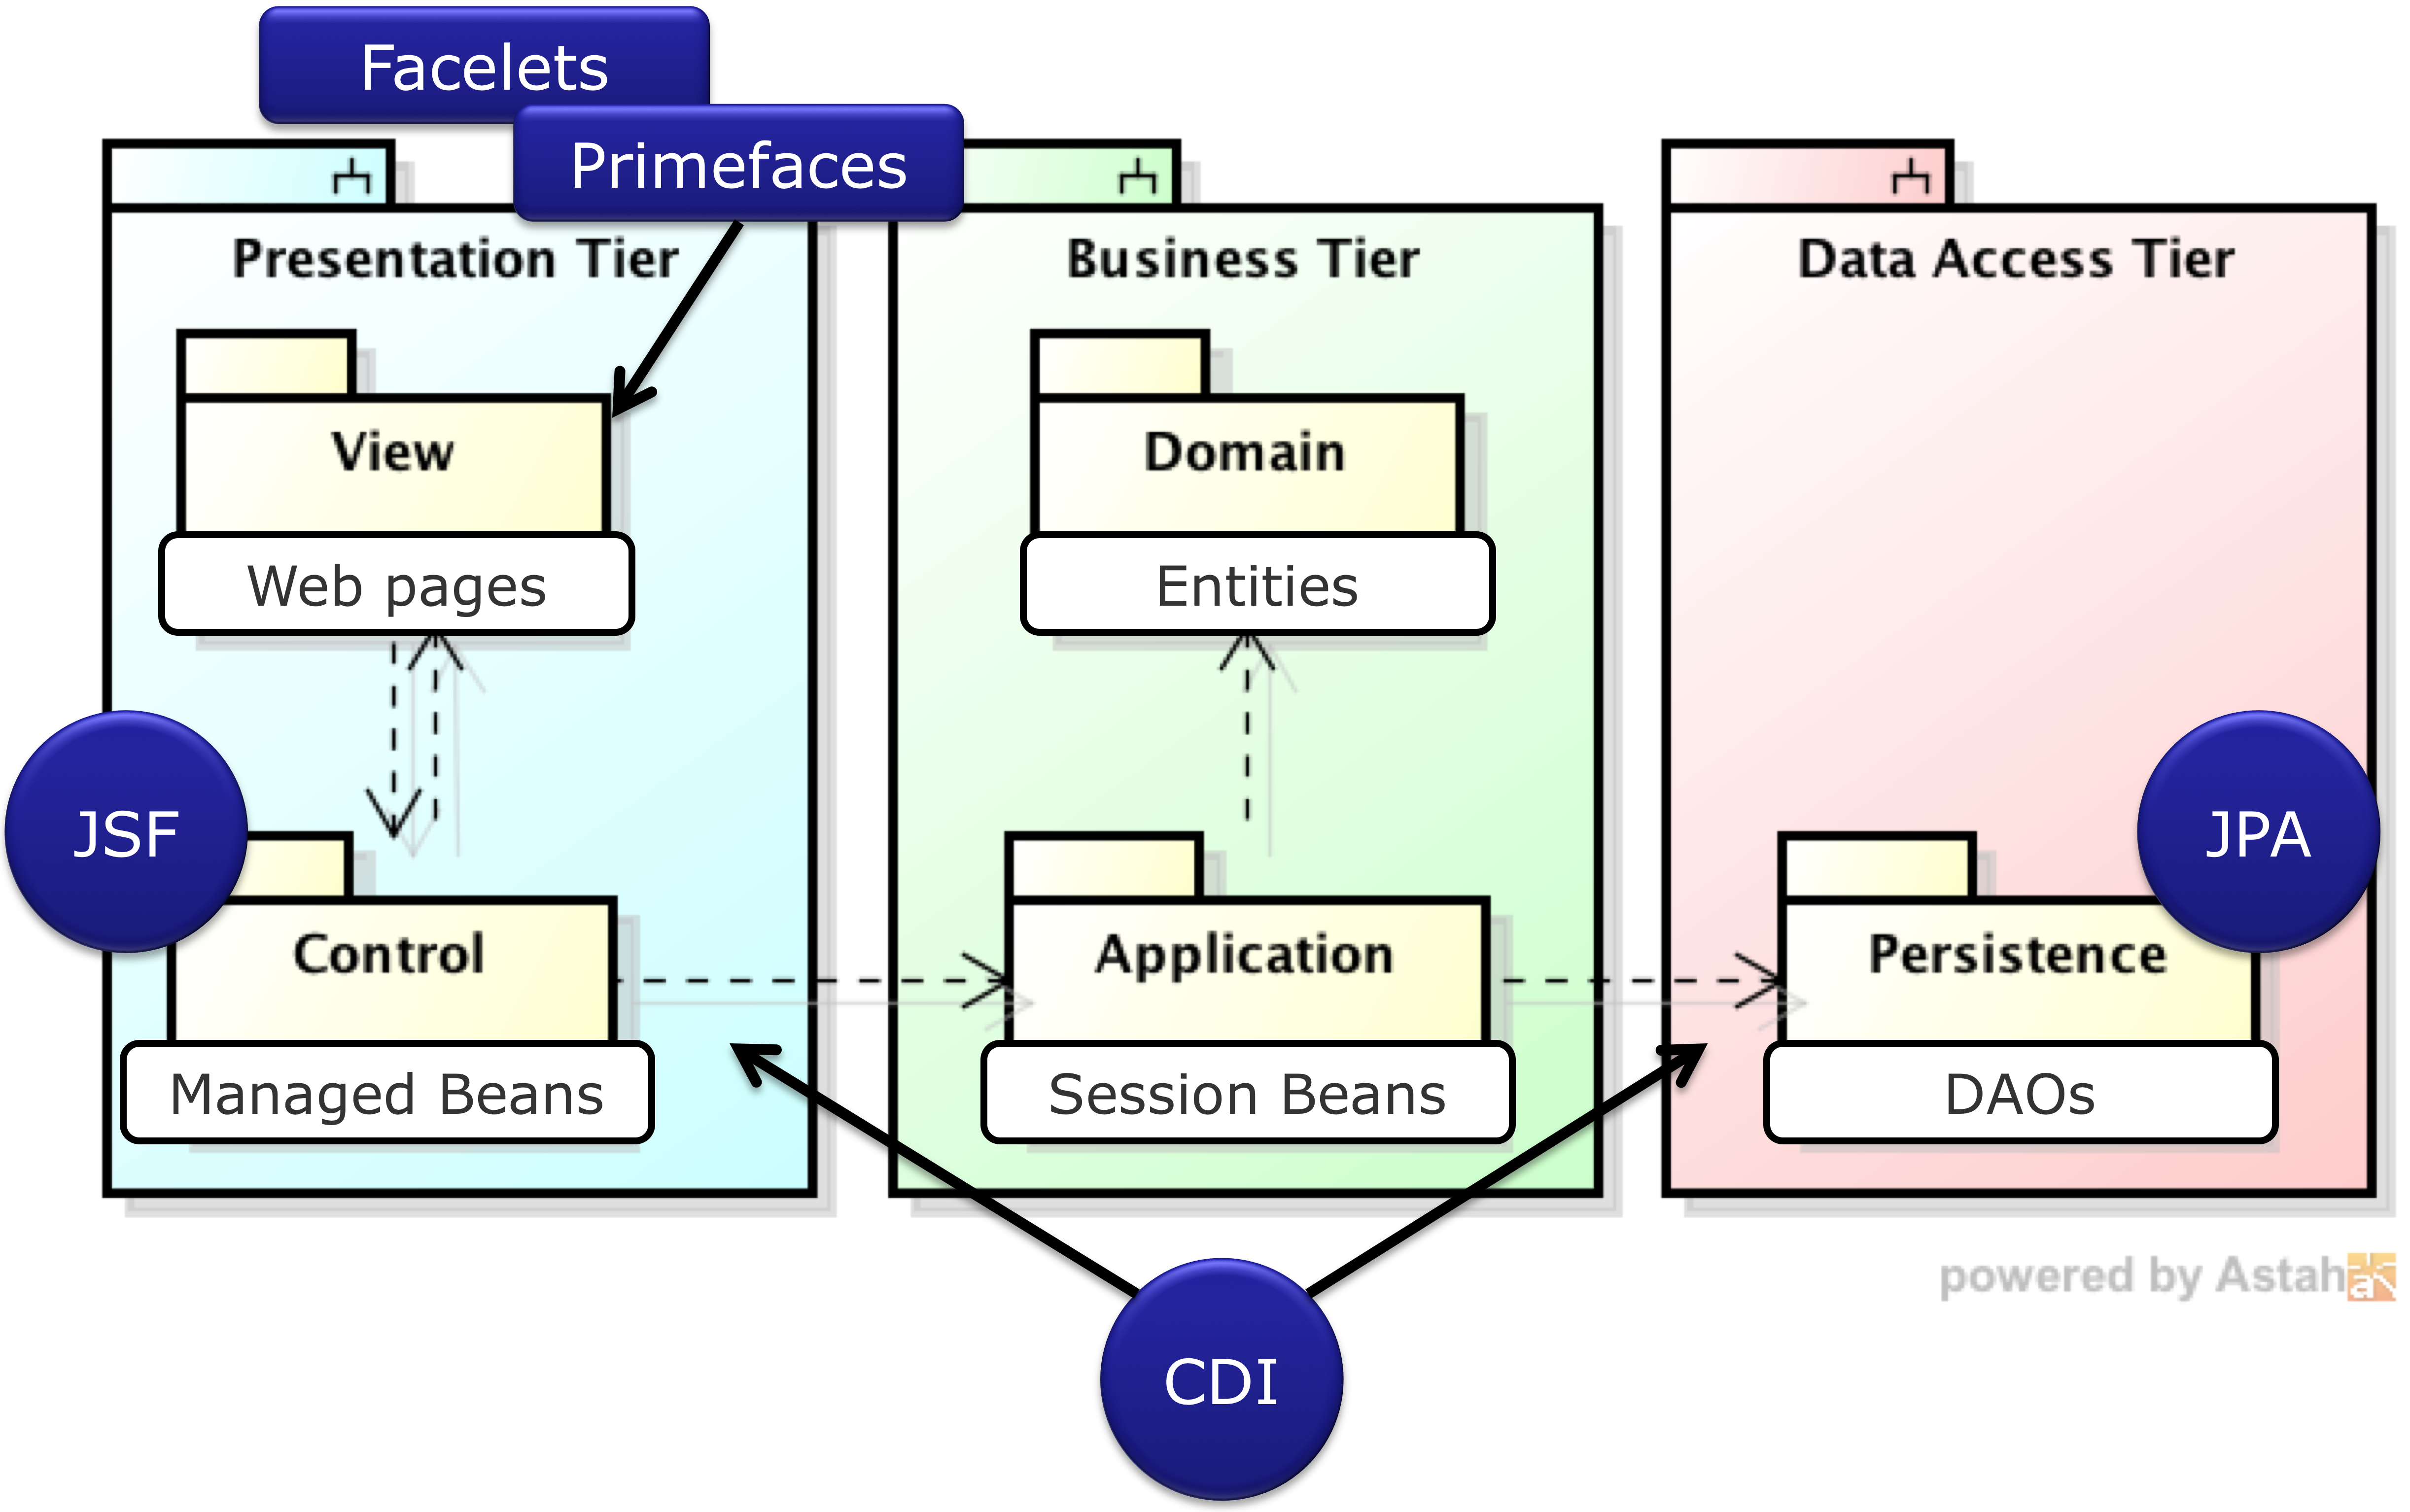
\includegraphics[width=0.7\textwidth]{figuras/figura-arquitetura-padrao.png}
	\caption{Arquitetura padrão proposta pelo FrameWeb.}
	\label{figura-arquitetura-padrao}
\end{figure}

Entretanto, como tal arquitetura não se mantém no padrão Django, que é composta de \textit{models}, \textit{views} e \textit{templates} com responsabilidades diferentes da dos elementos de mesmo nome na arquitetura Java EE. Portanto é necessario fazer aproximações para ambos os modelos dizerem a mesma coisa com palavras diferentes. Se adicionarmos uma camada de serviços entre os \textit{models} e \textit{views}, podemos obter uma arquitetura como a da figura \ref{figura-arquitetura-adaptada}, que é bastante similar à \ref{figura-arquitetura-padrao}. Como Django usa Active Record e não Data Access Objects, a camada de acesso ao dado foi ignorada.

\begin{figure}[h]
	\centering
	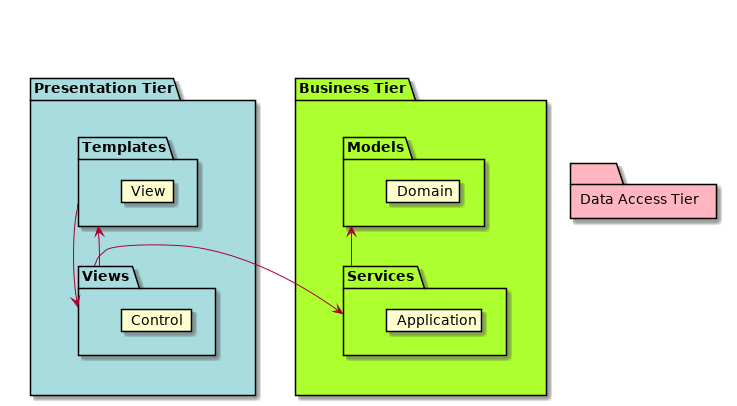
\includegraphics[width=0.7\textwidth]{figuras/arquitetura.png}
	\caption{Arquitetura que busca aproximar o modelo do Django à do FrameWeb.}
	\label{figura-arquitetura-adaptada}
\end{figure}

Nas próximas seções, serão apresentados diagramas FrameWeb relativos a cada uma das camadas da arquitetura do sistema.


\section{Camada de Apresentação}
\label{sec-arquitetura-apresentacao}

% \vitor{Apresentar os modelos de navegação do FrameWeb.}

\begin{figure}[H]
	\centering
	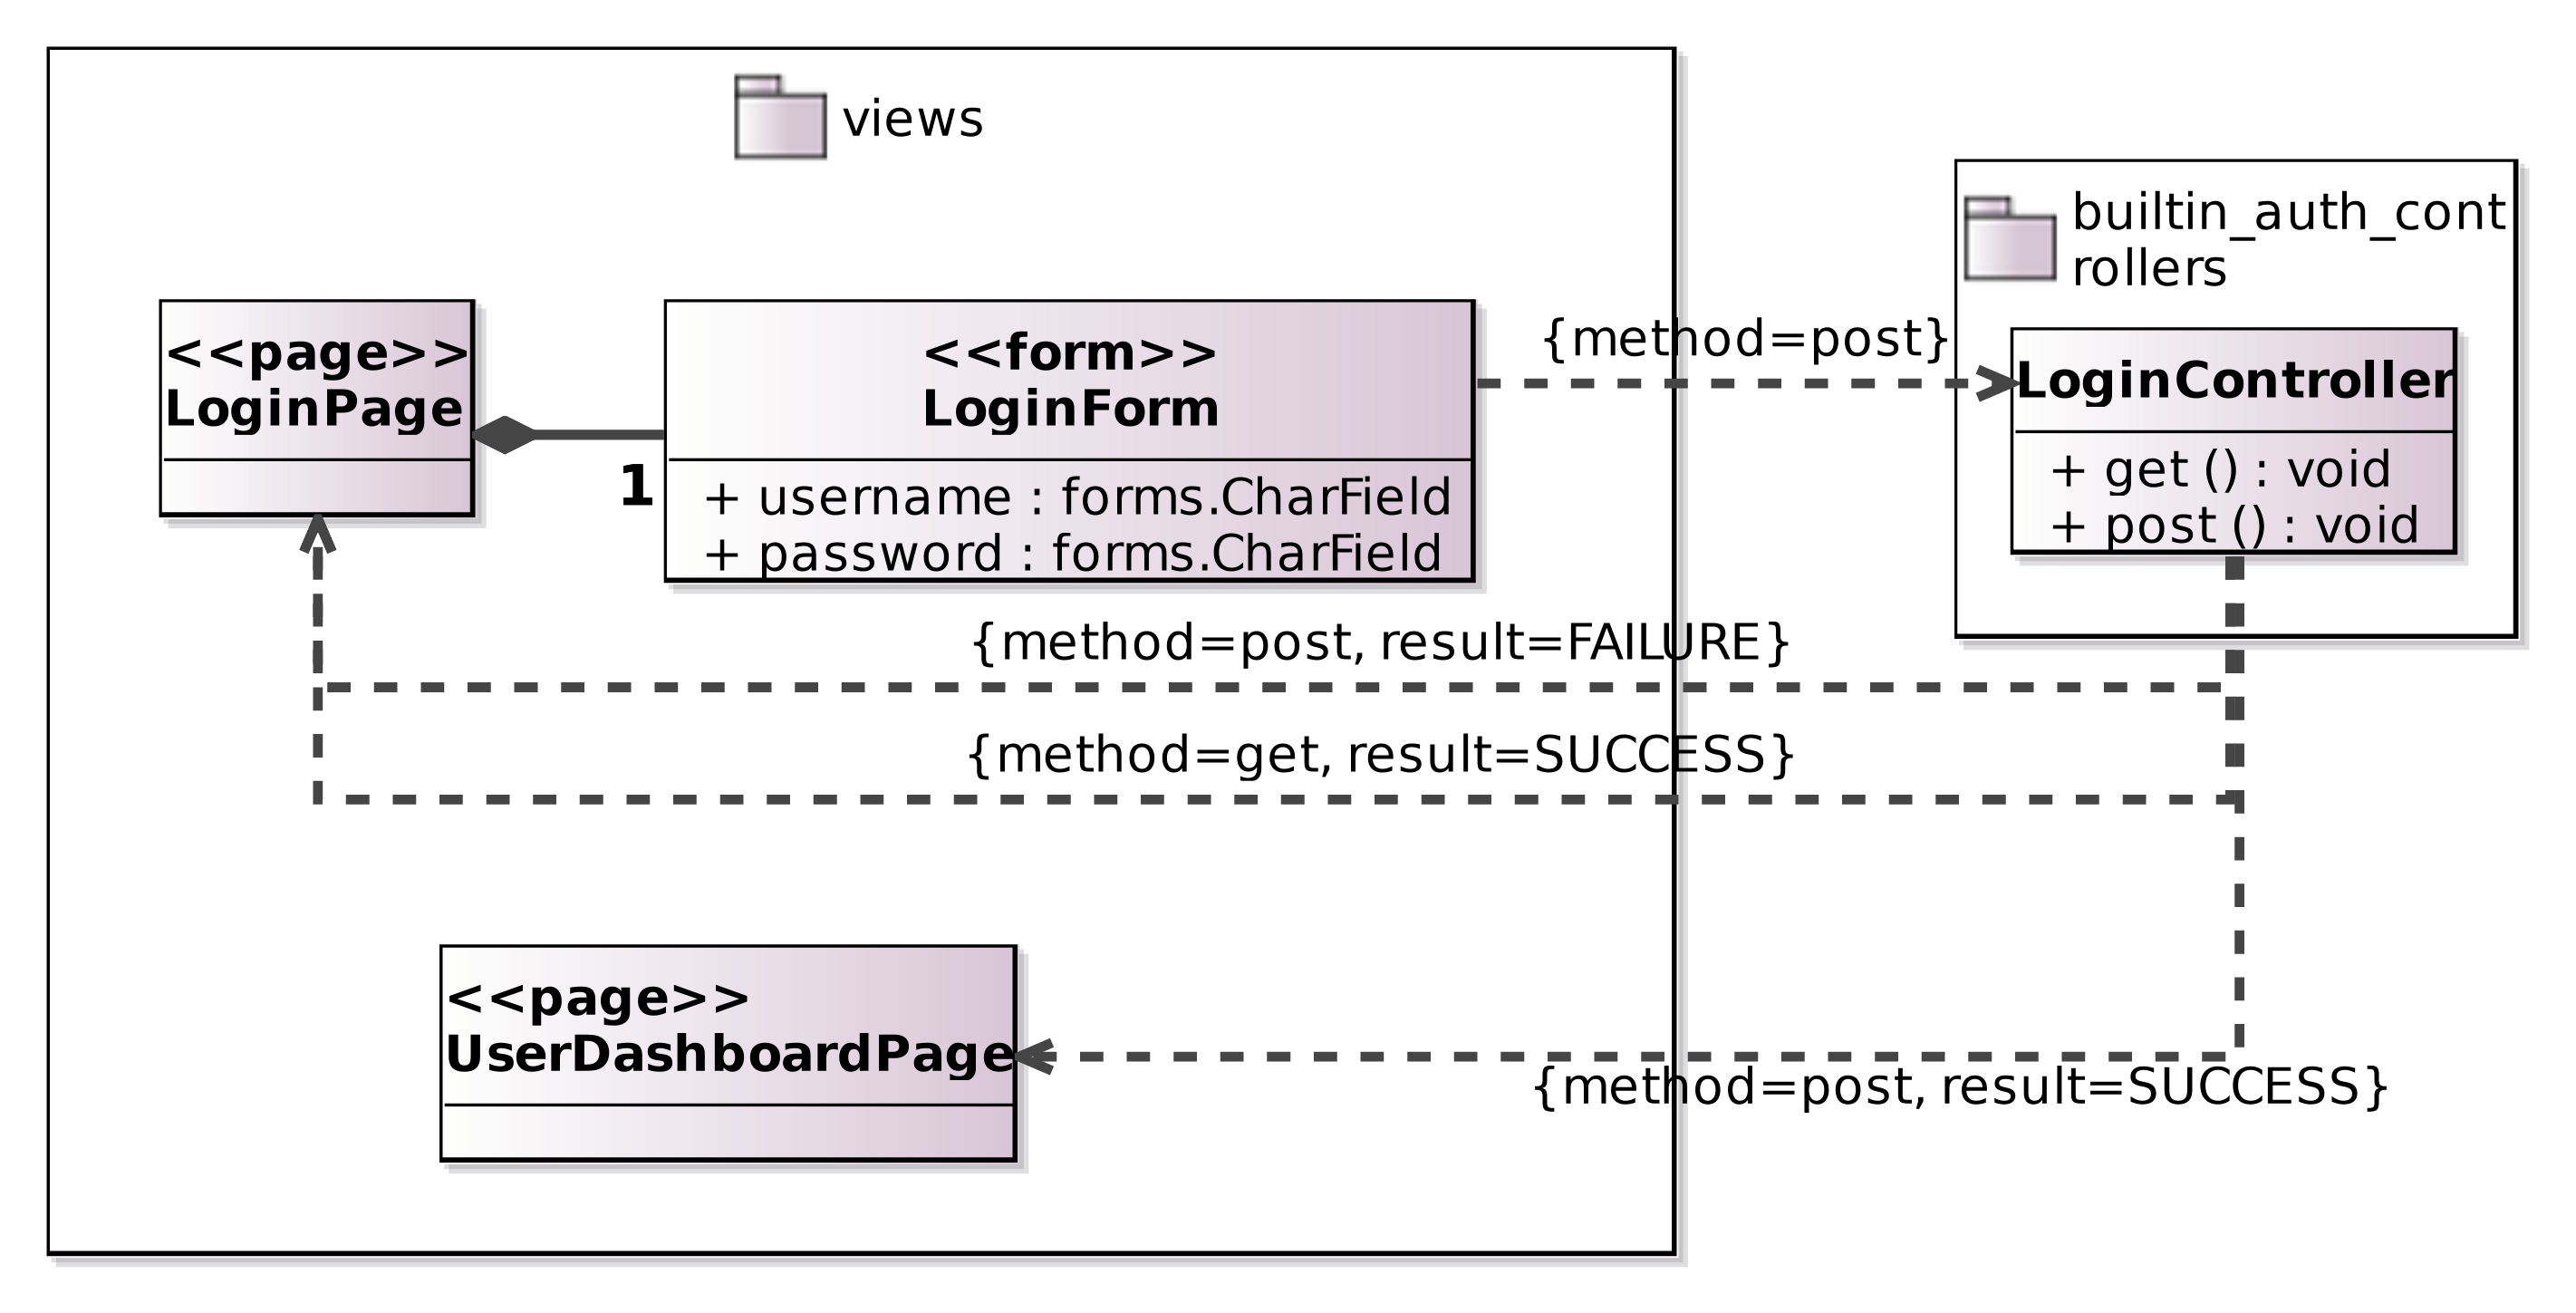
\includegraphics[scale=0.15]{figuras/FrameWebNavigationModel1.jpg}
	\caption{Modelo de Navegação do \imprimirtitulo{} -- Login}
	\label{fig:nav1}
\end{figure}

\begin{figure}[H]
	\centering
	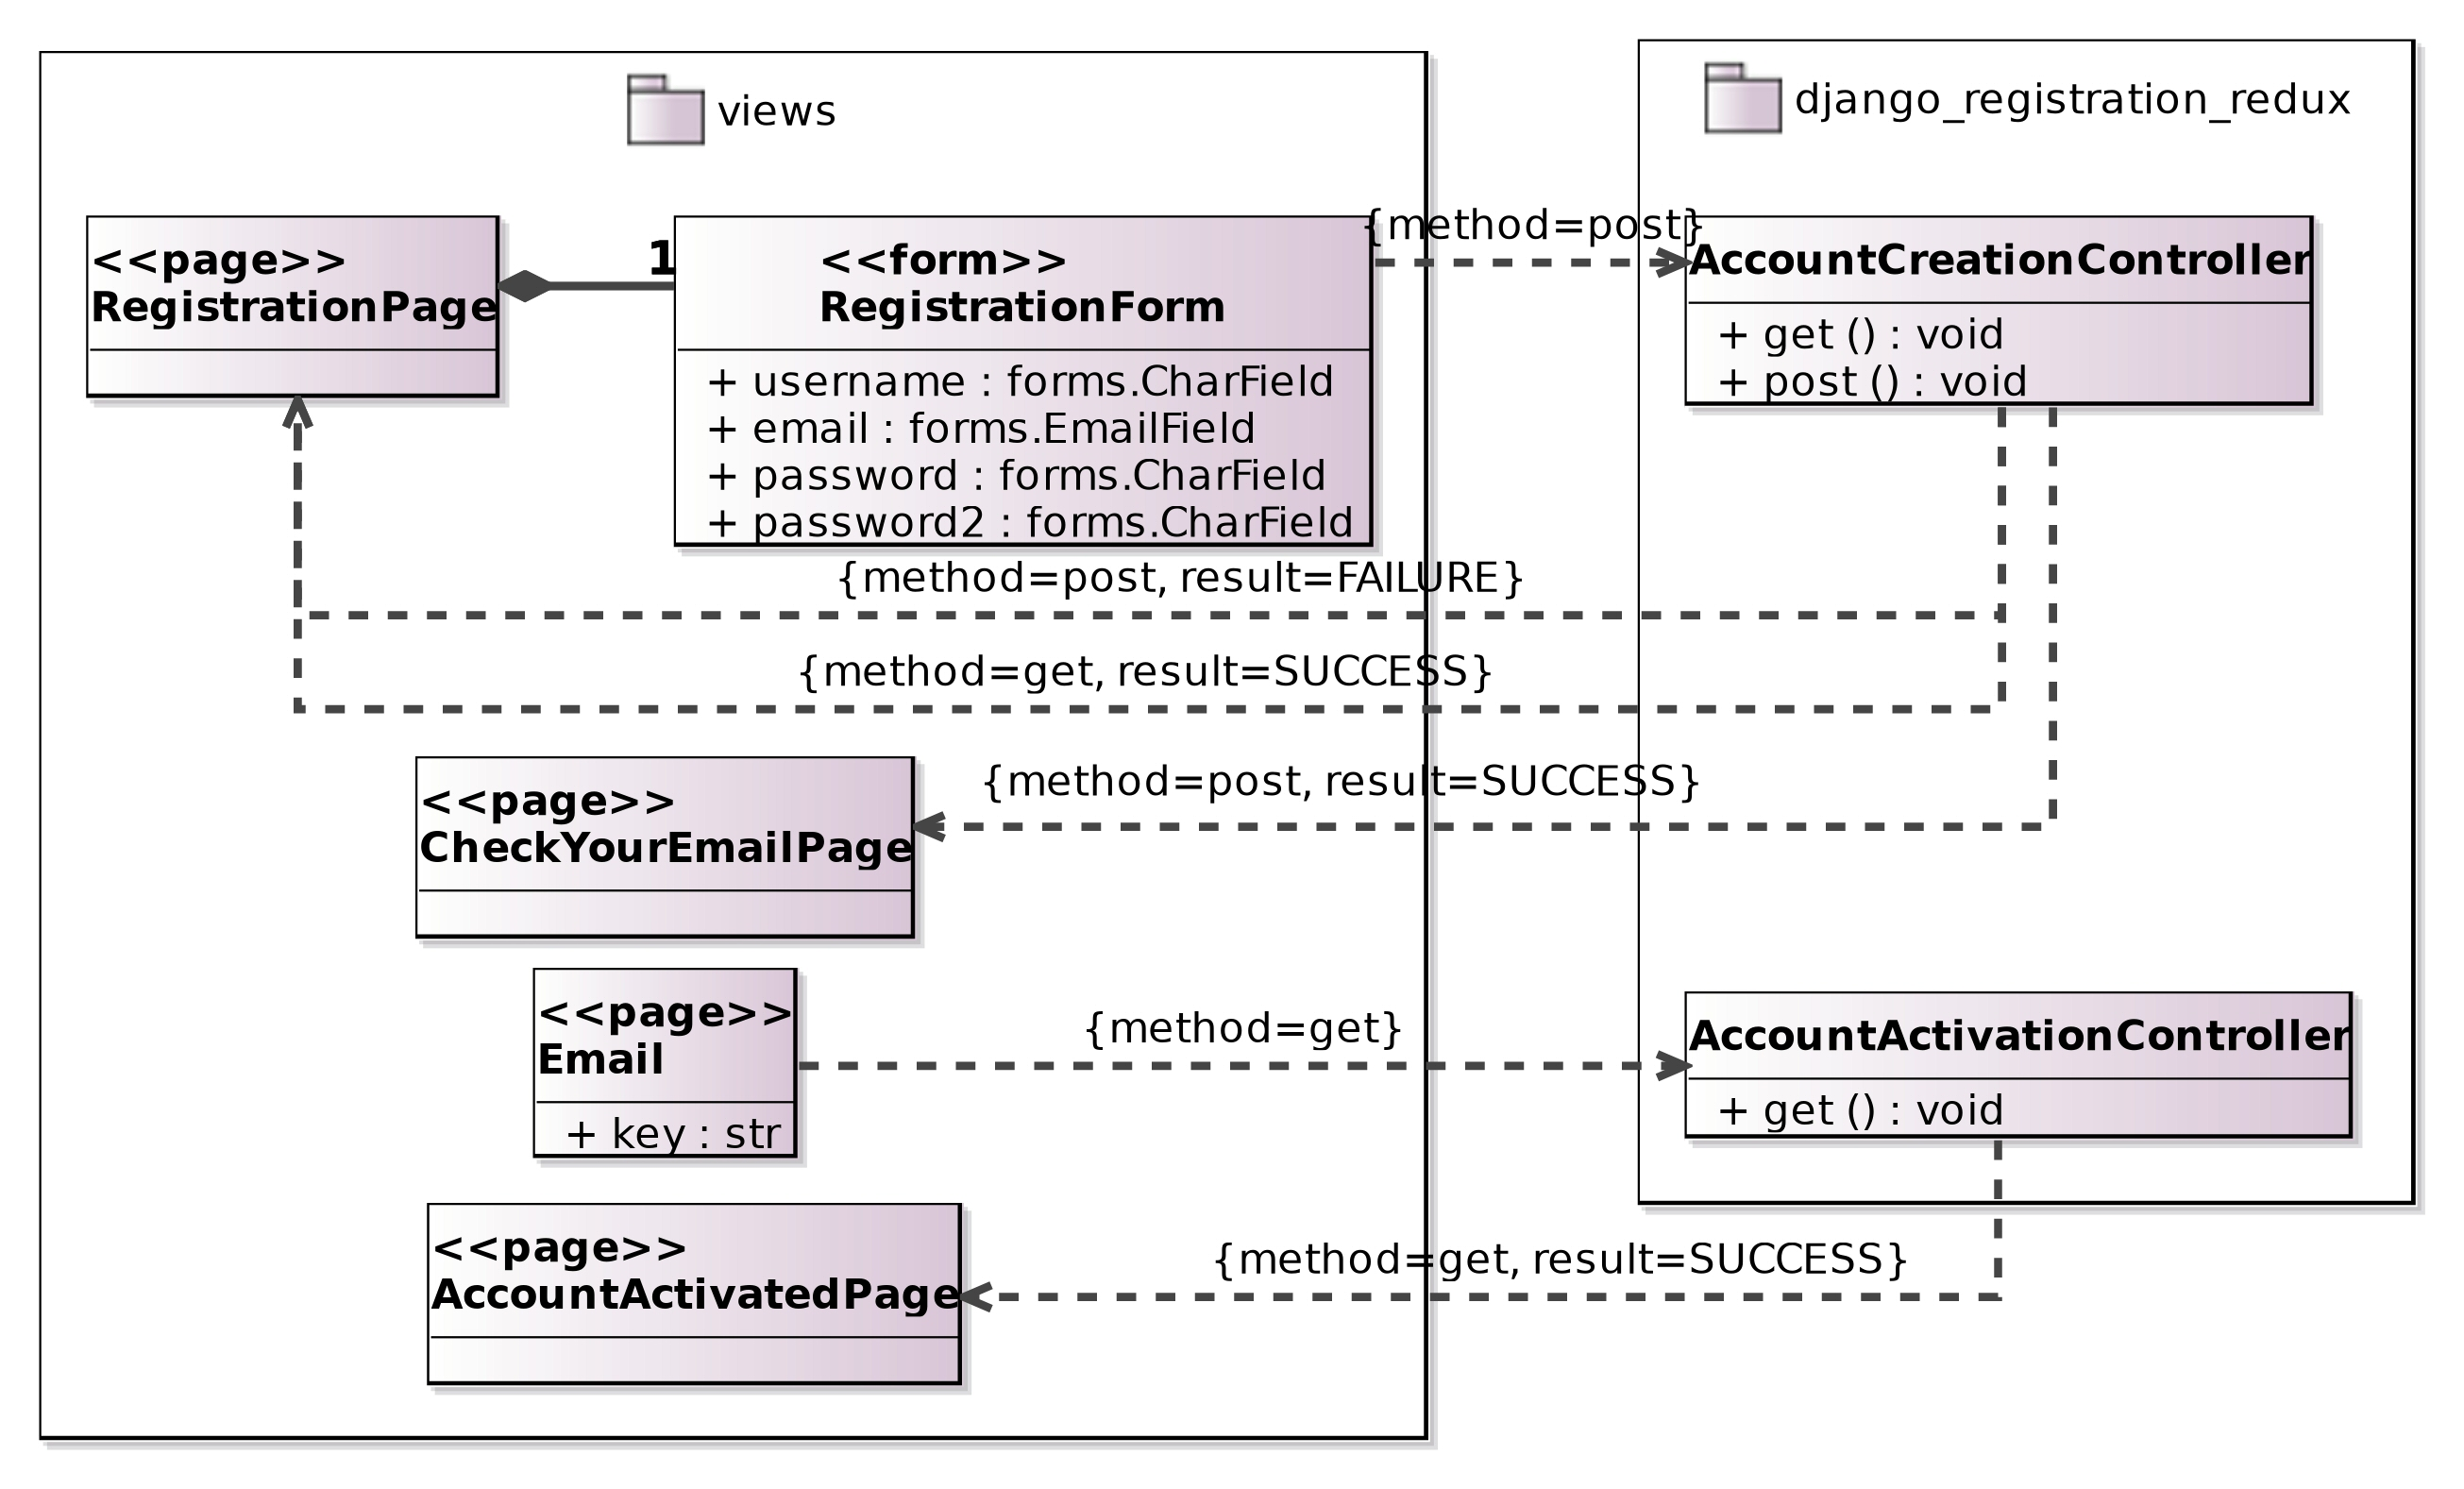
\includegraphics[scale=0.15]{figuras/FrameWebNavigationModel2.jpg}
	\caption{Modelo de Navegação do \imprimirtitulo{} -- Criar conta}
	\label{fig:nav2}
\end{figure}

\begin{figure}[H]
	\centering
	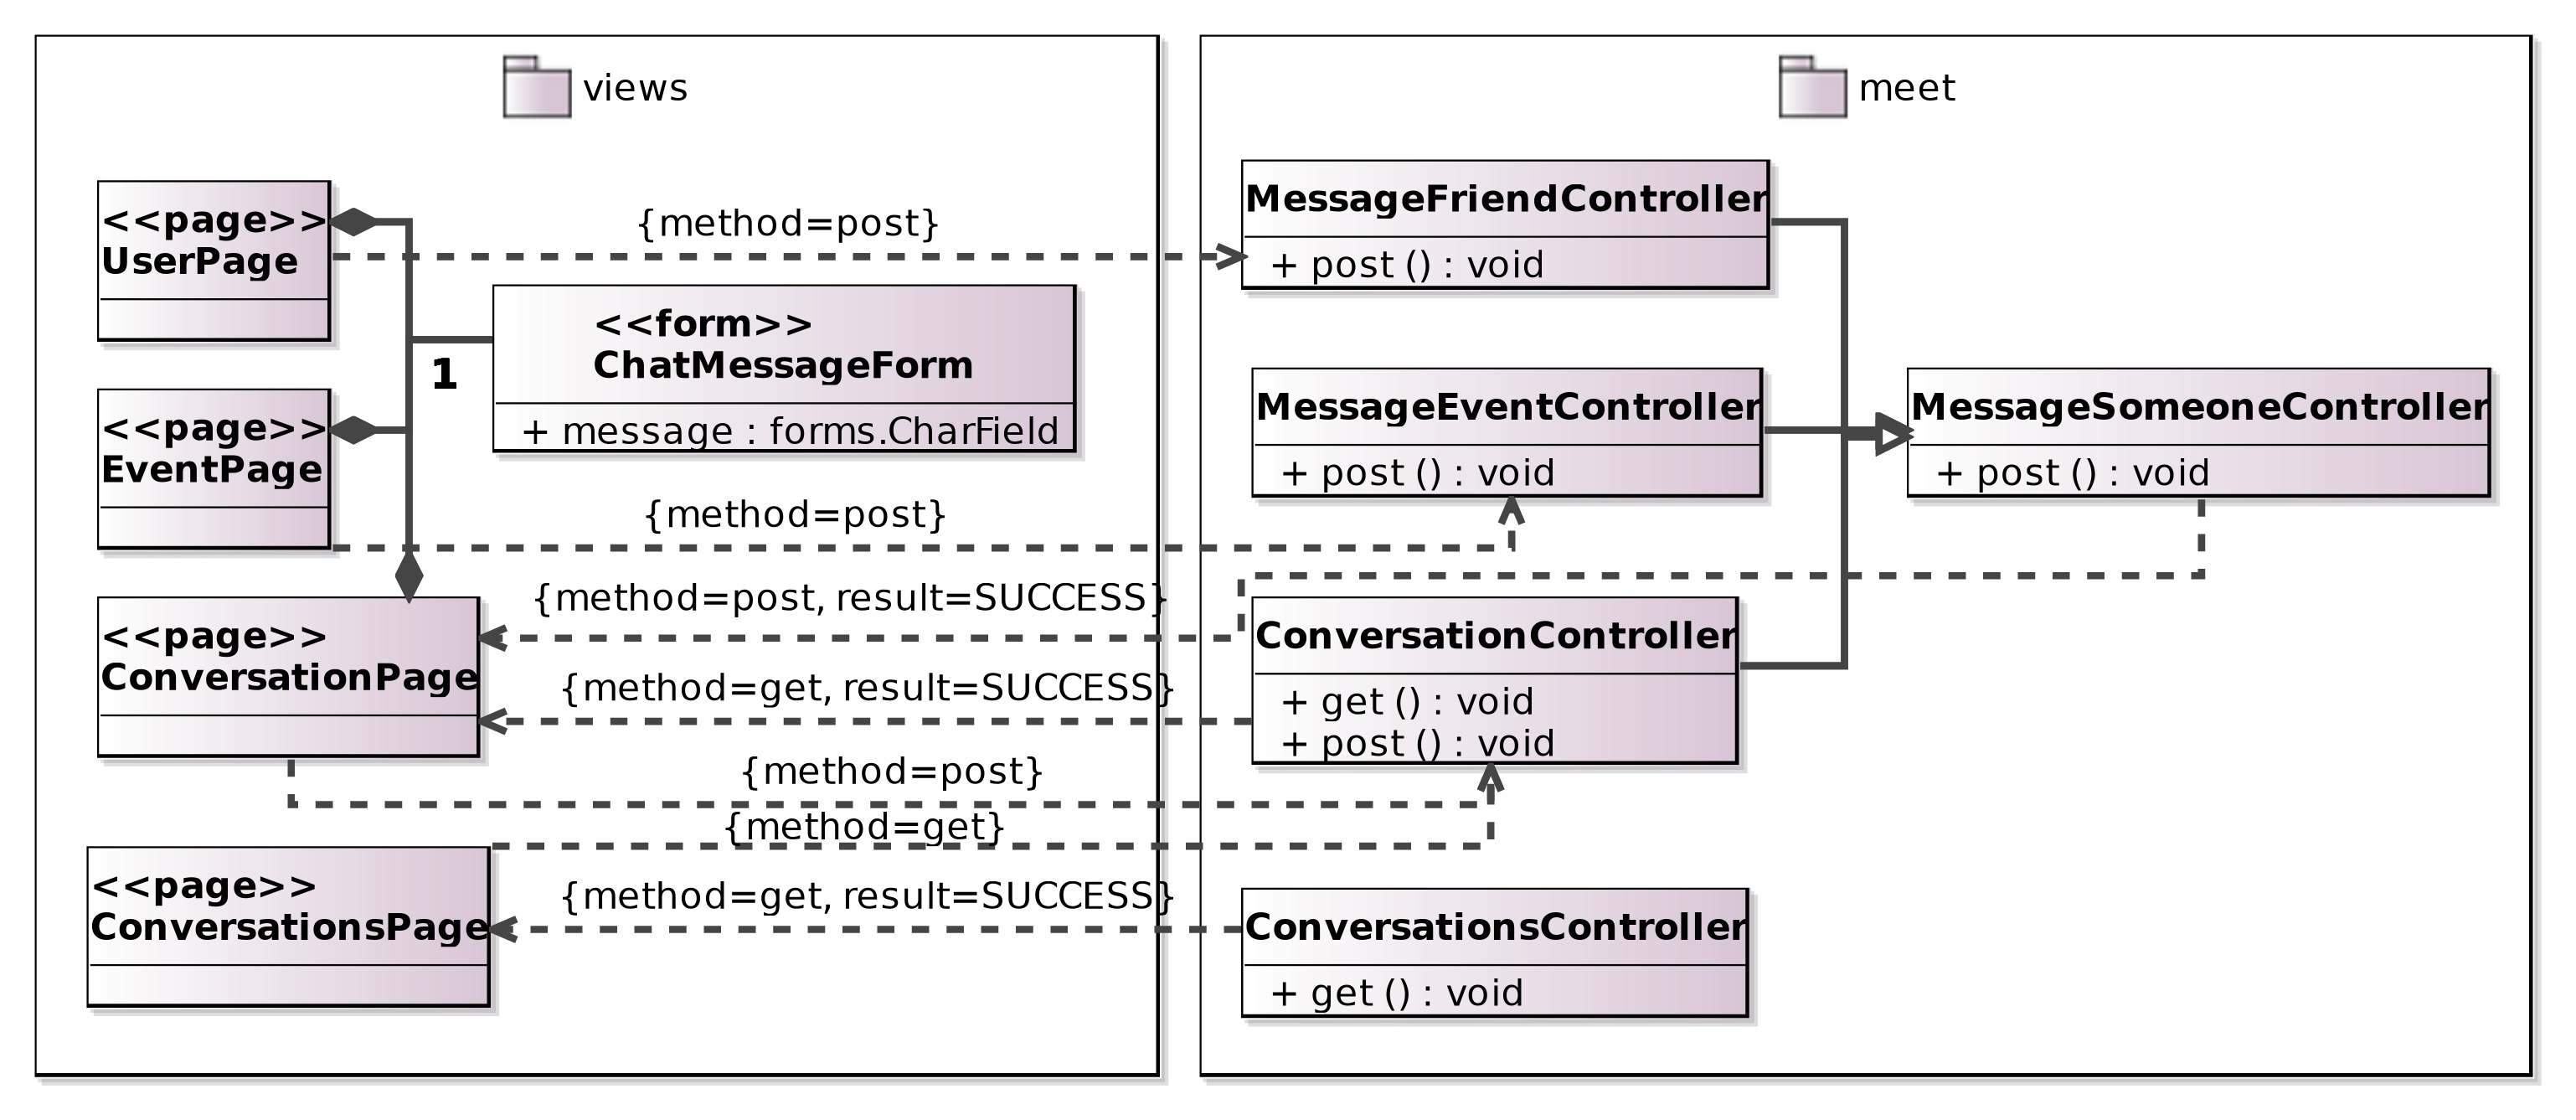
\includegraphics[scale=0.15]{figuras/FrameWebNavigationModel3.jpg}
	\caption{Modelo de Navegação do \imprimirtitulo{} -- Iniciar e continuar conversas}
	\label{fig:nav3}
\end{figure}

\begin{figure}[H]
	\centering
	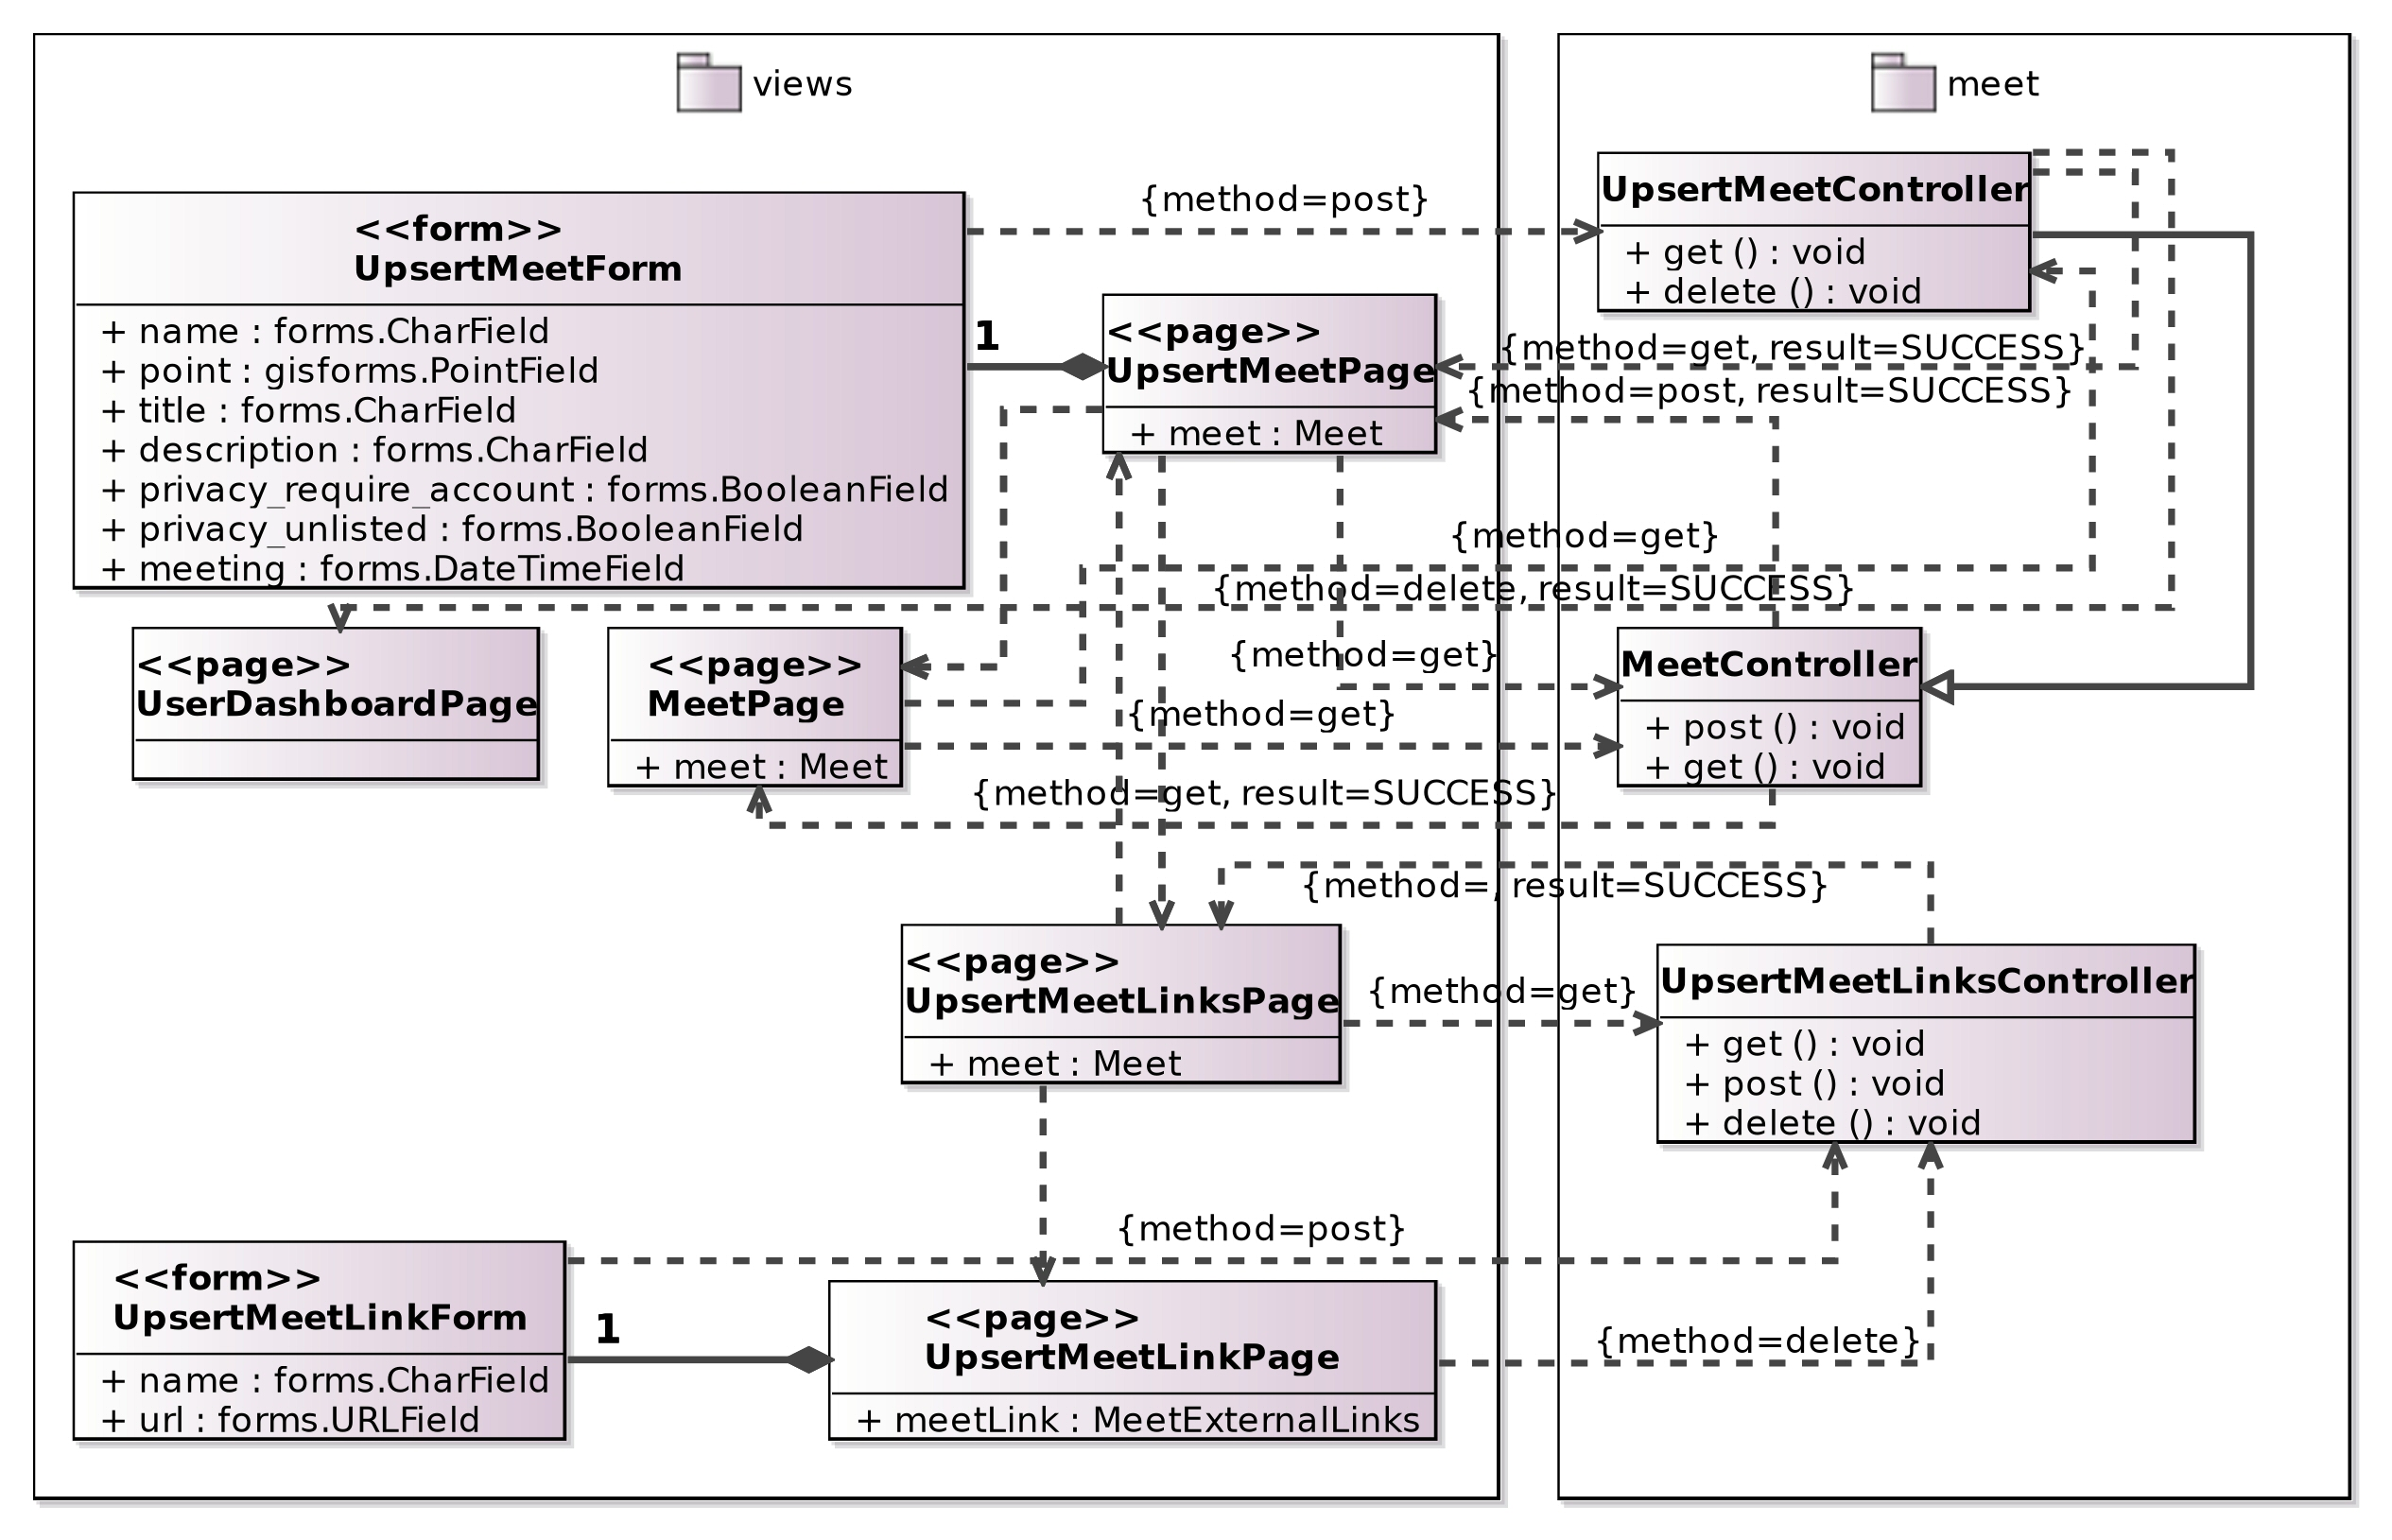
\includegraphics[scale=0.15]{figuras/FrameWebNavigationModel4.jpg}
	\caption{Modelo de Navegação do \imprimirtitulo{} -- Gerenciar encontros}
	\label{fig:nav4}
\end{figure}

\begin{figure}[H]
	\centering
	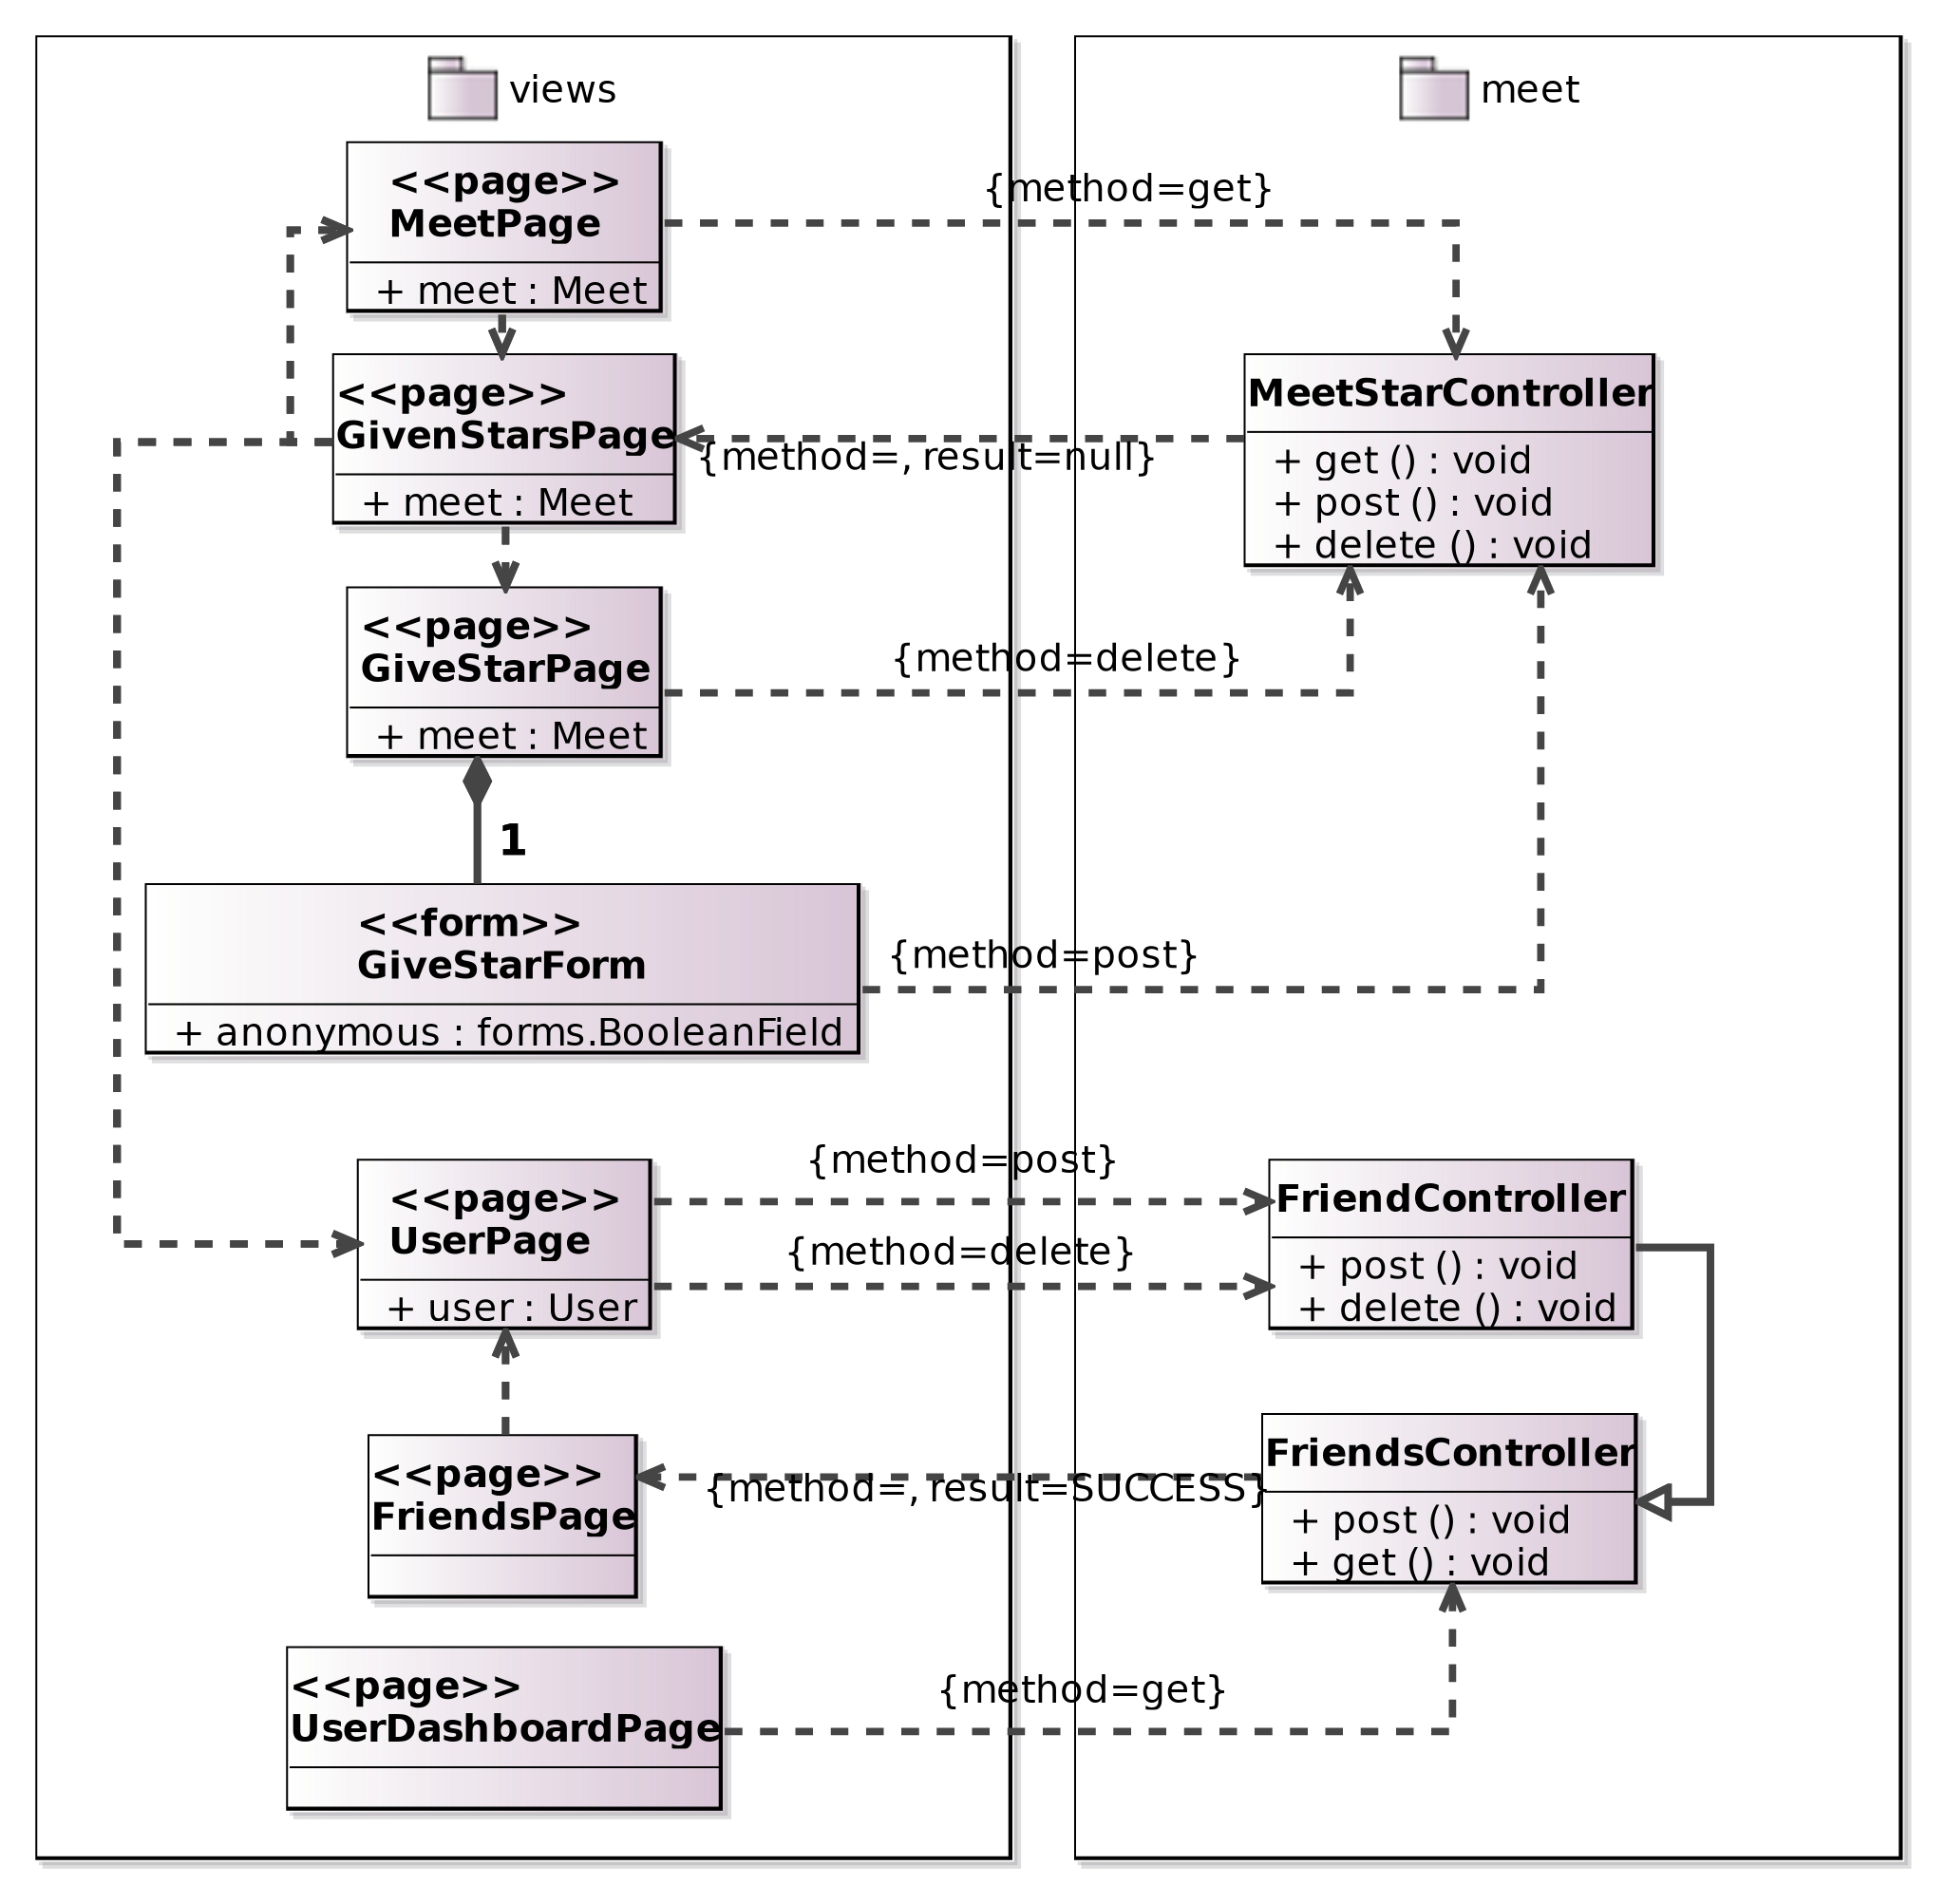
\includegraphics[scale=0.15]{figuras/FrameWebNavigationModel5.jpg}
	\caption{Modelo de Navegação do \imprimirtitulo{} -- Participar de encontros e adicionar/aceitar/rejeitar/desistir pedidos de amizade}
	\label{fig:nav5}
\end{figure}

\begin{figure}[H]
	\centering
	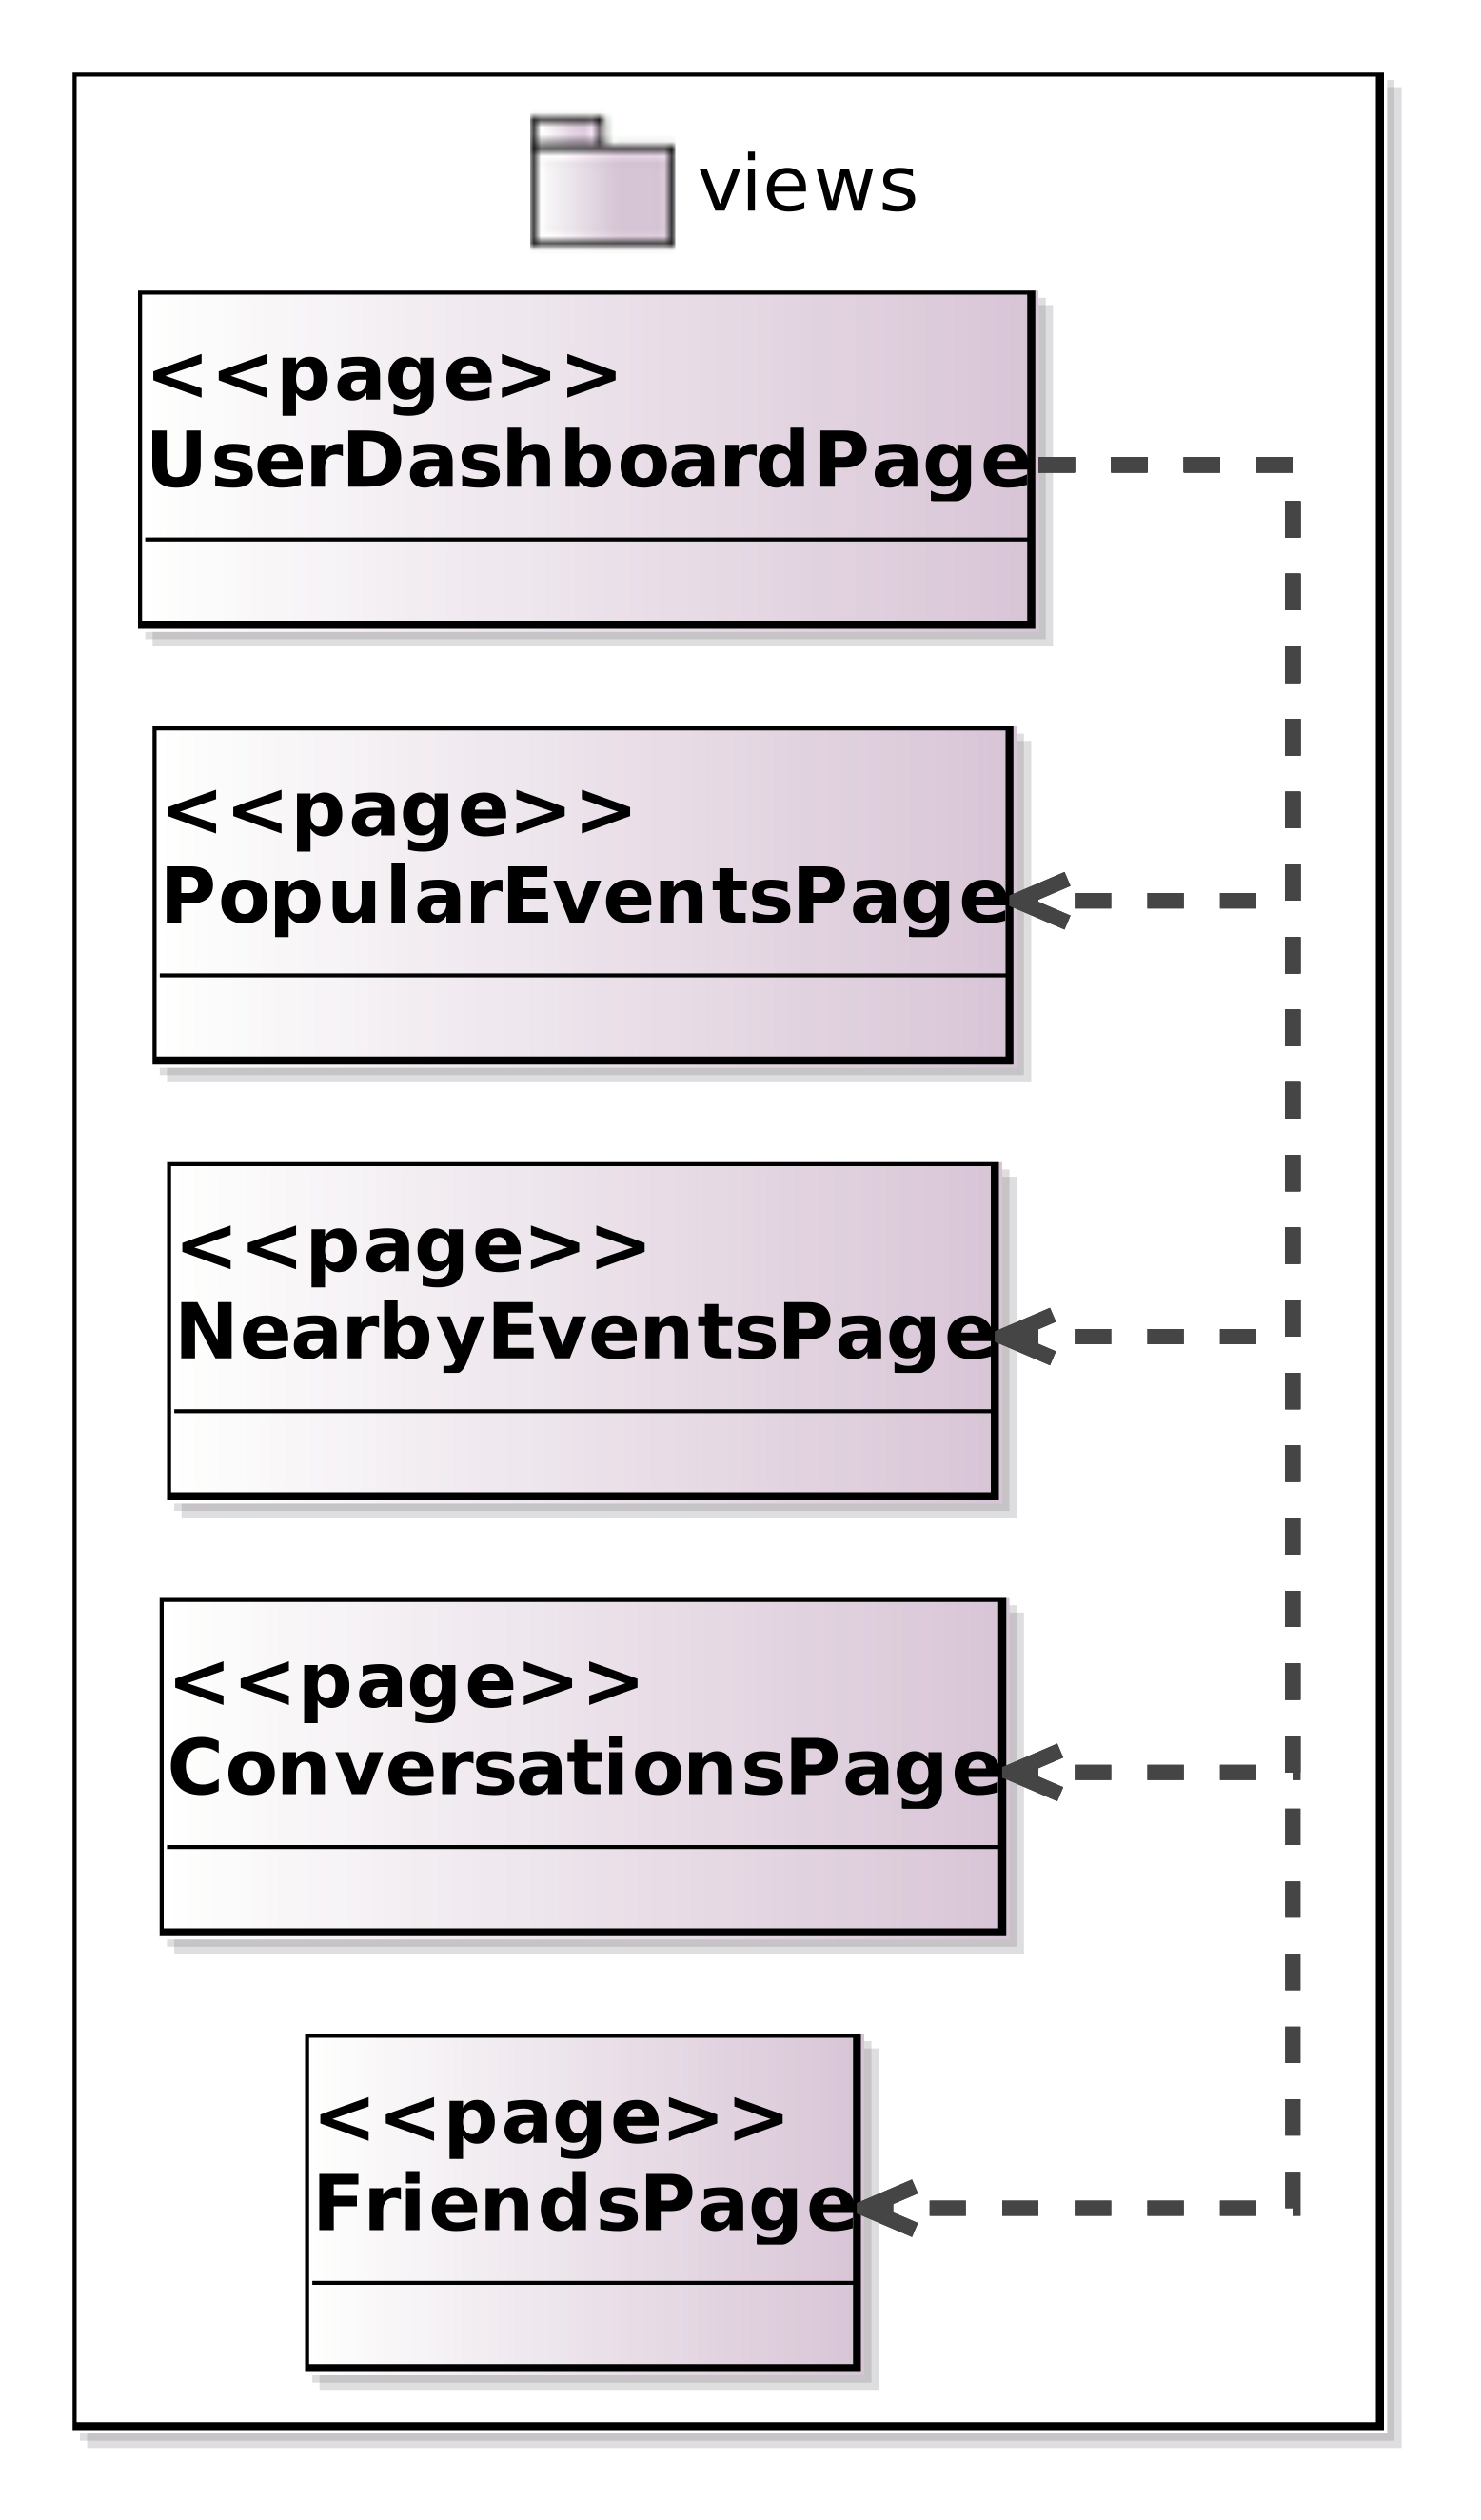
\includegraphics[scale=0.1]{figuras/FrameWebNavigationModel6.jpg}
	\caption{Modelo de Navegação do \imprimirtitulo{} -- O caminho do usuário de sua homepage até um ponto em comum com as funcionalidades mencionadas anteriormente; eventuais controladores foram omitidos}
	\label{fig:nav6}
\end{figure}




\section{Camada de Negócio}
\label{sec-arquitetura-negocio}

% \vitor{Apresentar os modelos de entidades e de aplicação do FrameWeb.}

\begin{figure}[H]
	\centering
	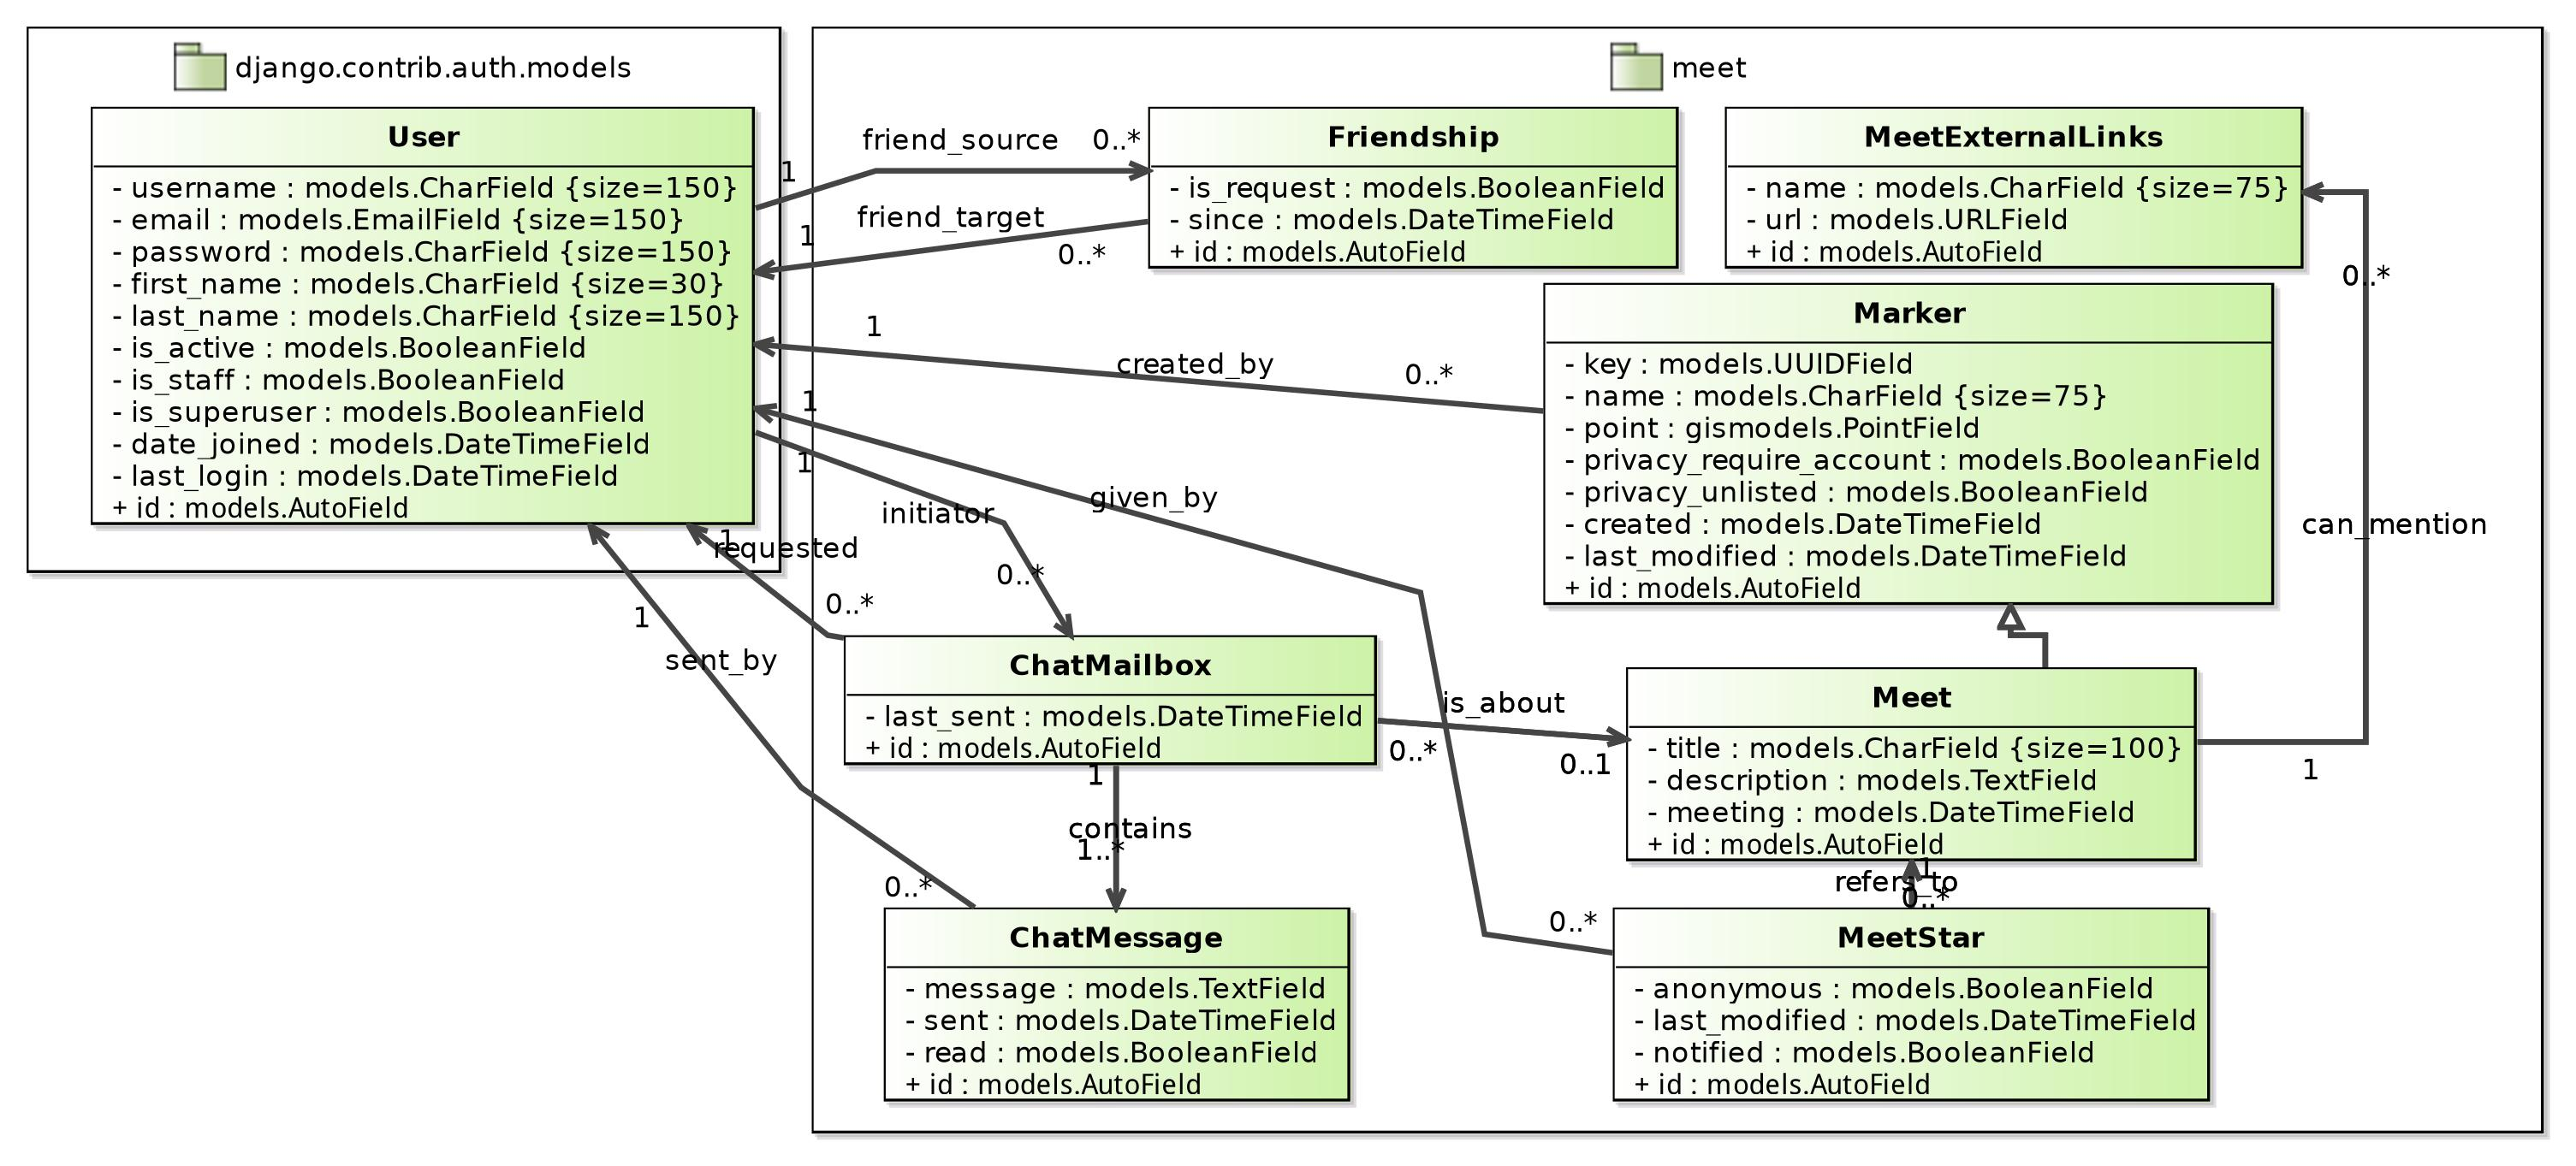
\includegraphics[width=0.8\textwidth]{figuras/FrameWebEntityModel.jpg}
	\caption{Modelo de Entidades do \imprimirtitulo.}
	\label{fig:ent}
\end{figure}

\begin{figure}[H]
	\centering
	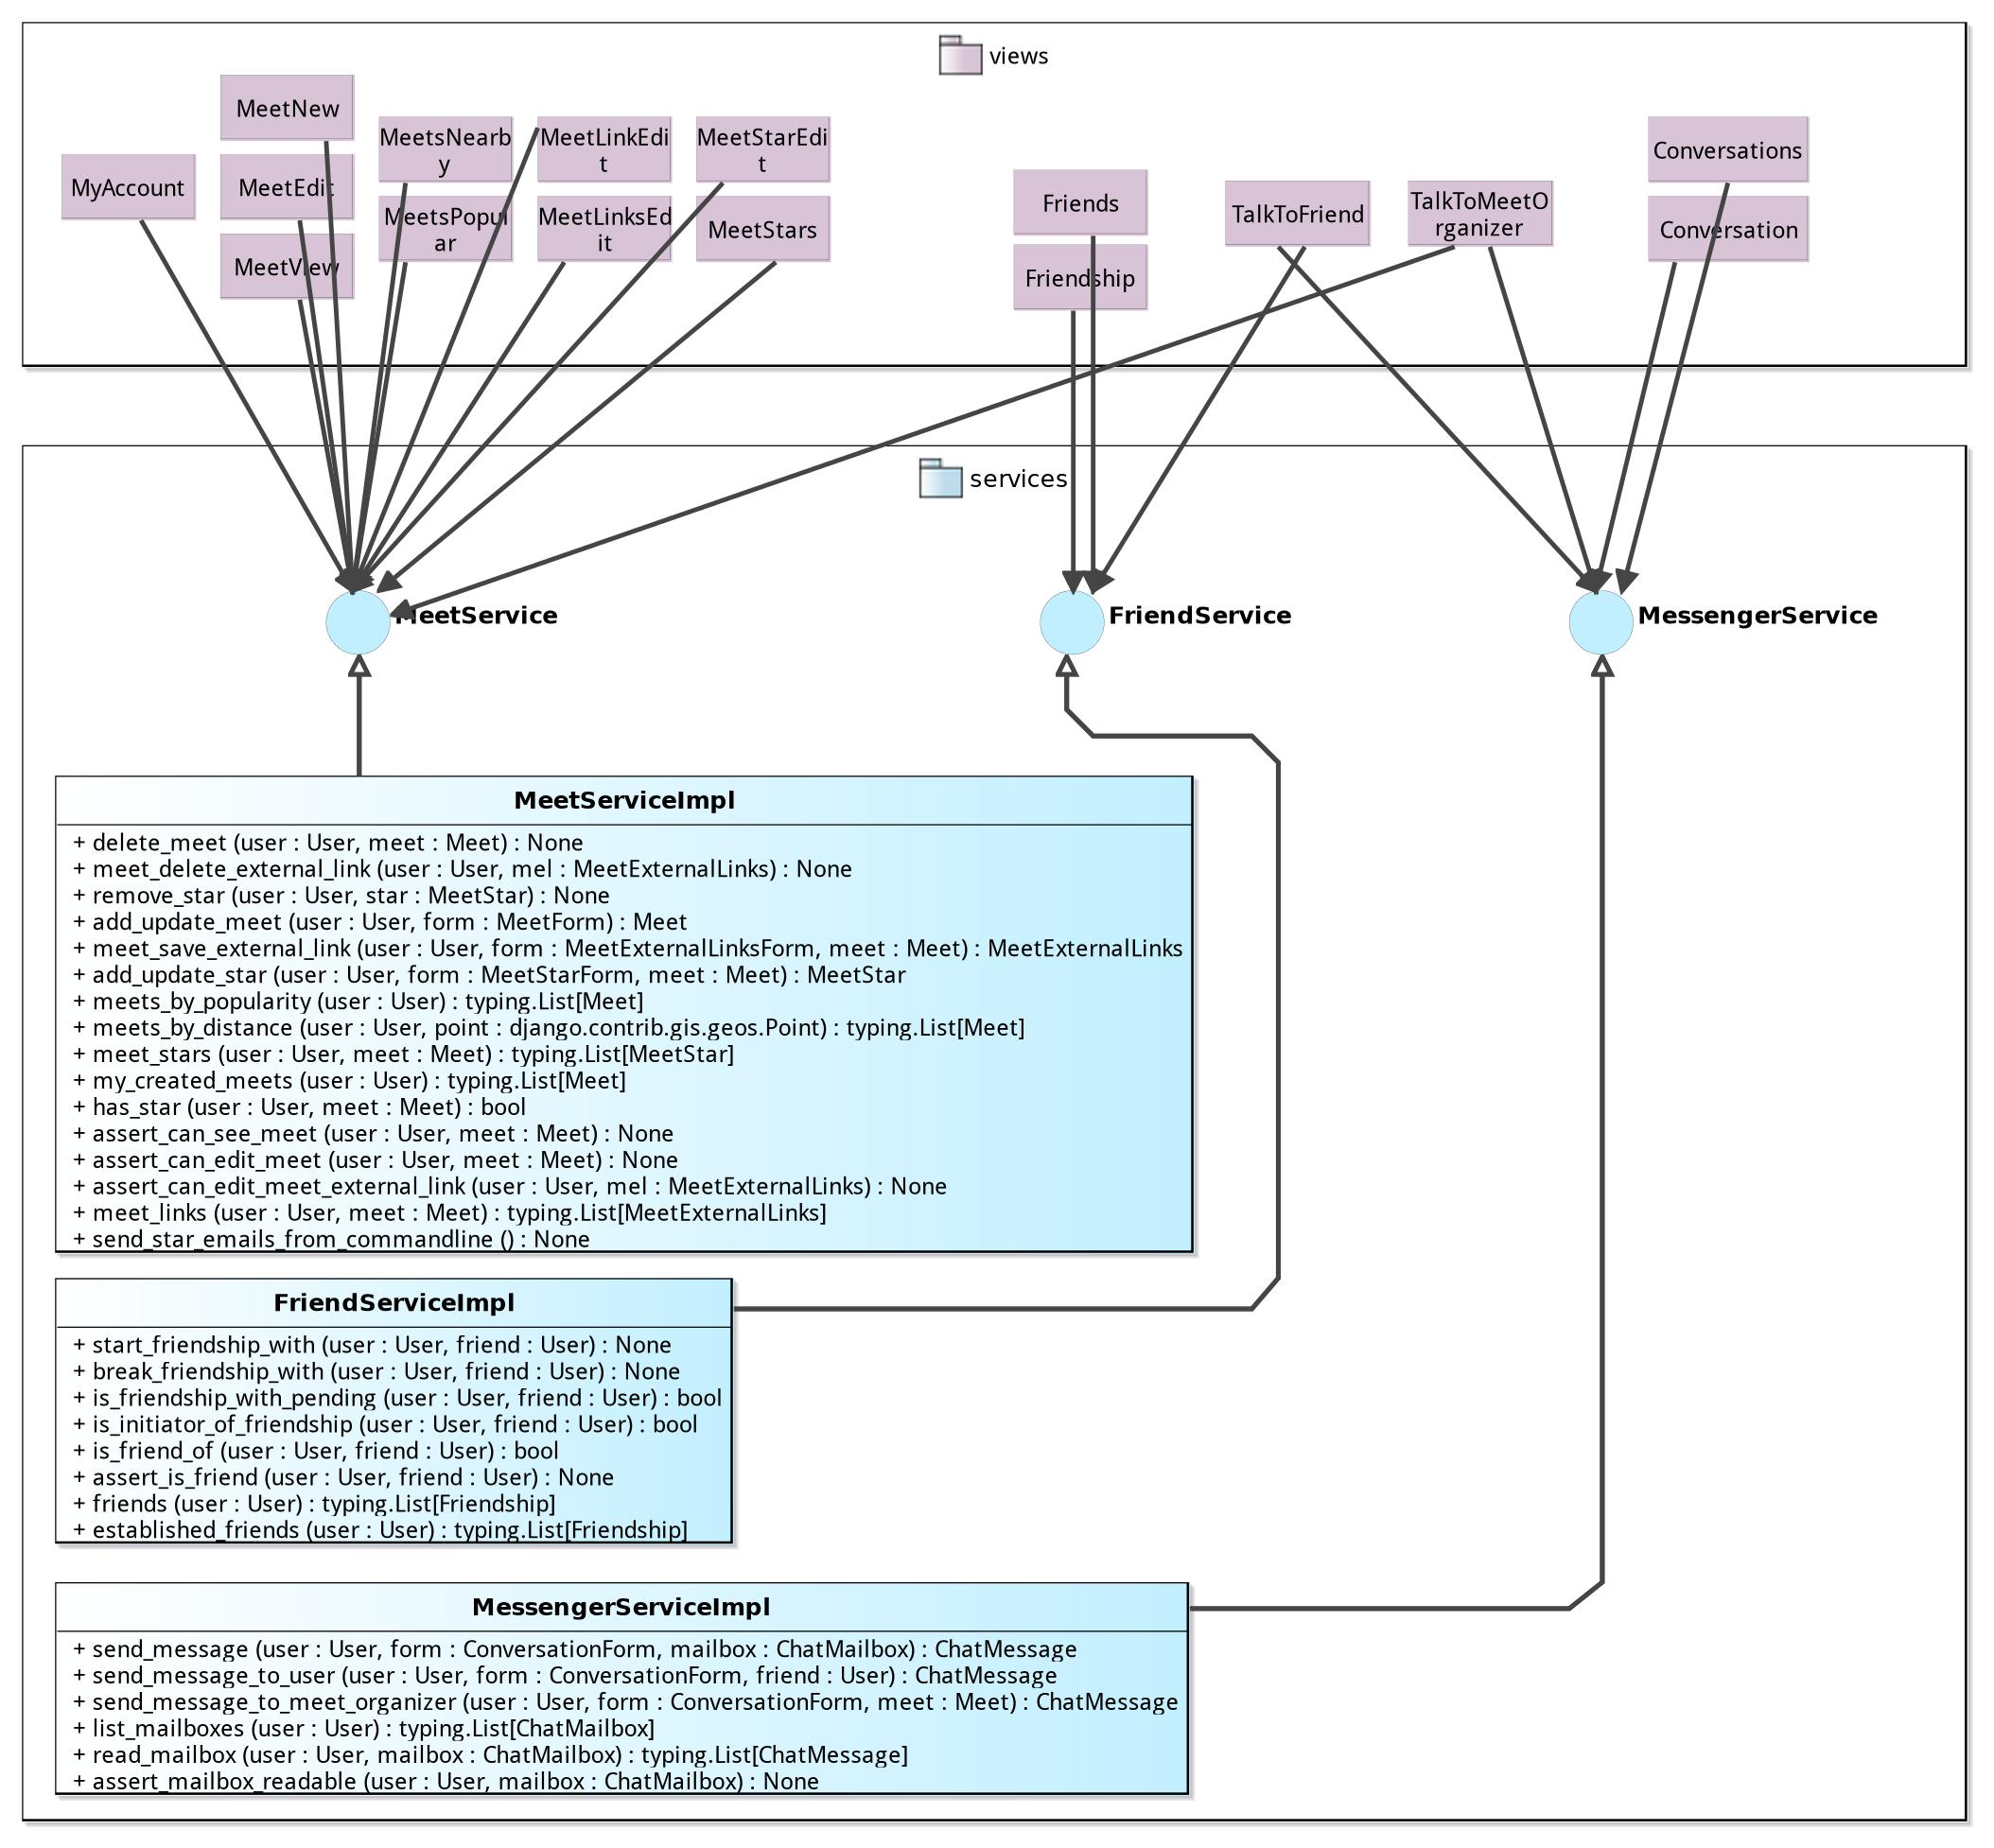
\includegraphics[width=0.8\textwidth]{figuras/FrameWebApplicationModel.jpg}
	\caption{Modelo de Aplicação do \imprimirtitulo.}
	\label{fig:apl}
\end{figure}




% \section{Camada de Acesso a Dados}
% \label{sec-arquitetura-dados}
%
% \vitor{Apresentar os modelos de persistência do FrameWeb.}




%%% Páginas finais do documento: bibliografia e anexos. %%%
% Finaliza a parte no bookmark do PDF para que se inicie o bookmark na raiz e adiciona espaço de parte no sumário.
\phantompart

% Marca o início dos elementos pós-textuais.
\postextual

% Referências bibliográficas
\bibliography{bibliografia}

% Índice remissivo.
\phantompart
\printindex

% Fim do documento.
\end{document}
